\documentclass[a4paper,12pt]{report} % добавить leqno в [] для нумерации слева

%%% Работа с русским языком
\usepackage{cmap}					% поиск в PDF
\usepackage{mathtext} 				% русские буквы в формулах
\usepackage[T2A]{fontenc}			% кодировка
\usepackage[utf8]{inputenc}			% кодировка исходного текста
\usepackage[english,russian]{babel}	% локализация и переносы

\usepackage{graphicx}				%вставка изображений(графиков, в частности)
\usepackage{listings}
\usepackage{color}

\definecolor{dkgreen}{rgb}{0,0.6,0}
\definecolor{gray}{rgb}{0.5,0.5,0.5}
\definecolor{mauve}{rgb}{0.58,0,0.82}

\lstset{frame=tb,
  language=Python,
  aboveskip=3mm,
  belowskip=3mm,
  showstringspaces=false,
  columns=flexible,
  basicstyle={\small\ttfamily},
  numbers=none,
  numberstyle=\tiny\color{gray},
  keywordstyle=\color{blue},
  commentstyle=\color{dkgreen},
  stringstyle=\color{mauve},
  breaklines=true,
  breakatwhitespace=true,
  tabsize=4
}

%%% Дополнительная работа с математикой
\usepackage{amsmath,amsfonts,amssymb,amsthm,mathtools} % AMS
\usepackage{icomma} % "Умная" запятая: $0,2$ --- число, $0, 2$ --- перечисление

%% Номера формул
\mathtoolsset{showonlyrefs=true} % Показывать номера только у тех формул, на которые есть \eqref{} в тексте.

%% Шрифты
\usepackage{euscript}	 % Шрифт Евклид
\usepackage{mathrsfs} % Красивый матшрифт

%% Свои команды
\DeclareMathOperator{\sgn}{\mathop{sgn}}

%\setlength\parindent{0ex}
%\setlength\parskip{0.3cm}

\renewcommand{\arraystretch}{1.8}

%%% Заголовок
\author{Волков Павел А-14-19}
\title{Отчет по Лабораторной работе №4}
\date{\today}

\begin{document}

\begin{titlepage}
	\newpage

	\begin{center}
	НАЦИОНАЛЬНЫЙ ИССЛЕДОВАТЕЛЬСКИЙ УНИВЕРСИТЕТ\\
		"МОСКОВСКИЙ ЭНЕРГЕТИЧЕСКИЙ ИНСТИТУТ"\\
	\end{center}

	\vspace{8em}	

	\begin{center}
		\Large Кафедра математического и компьютерного моделирования\\ 
	\end{center}

	\vspace{2em}

	\begin{center}
		\textsc{\textbf{ \Large Численные методы \linebreak Отчет по лабораторной работе №5 \linebreak "Численное интегрирование." \linebreak Вариант 52}}
	\end{center}

	\vspace{6em}



	\newbox{\lbox}
	\savebox{\lbox}{\hbox{Амосова Ольга Алексеевна}}
	\newlength{\maxl}
	\setlength{\maxl}{\wd\lbox}
	\hfill\parbox{11cm}{
		\hspace*{5cm}\hspace*{-5cm}Студент:\hfill\hbox to\maxl{Волков Павел Евгеньевич\hfill}\\
		\hspace*{5cm}\hspace*{-5cm}Преподаватель:\hfill\hbox to\maxl{Амосова Ольга Алексеевна}\\
		\\
		\hspace*{5cm}\hspace*{-5cm}Группа:\hfill\hbox to\maxl{А-14-19}\\
	}


	\vspace{\fill}

	\begin{center}
		Москва \\2021
	\end{center}

\end{titlepage}
\section*{Задача 4.1}
\subsection*{Постановка задачи}
В таблице приведены данные о численности населения некоторых
крупнейших стран мира по годам с 1950-2000 г.г. Заполнить последние два столбца
таблицы (взять сведения из интернета). На основе этих данных для конкретного варианта
построить наилучший многочлен по МНК. Найти численность населения страны в 2019
году и сравнить полученное значение с актуальным значением (взять из интернета).
Решить ту же задачу на основе интерполяционного многочлена. То есть построить
интерполяционный многочлен по значениям с 1950-2020 г.г. Вычислить значение для
2019 года и сравнить с актуальными данными.

\begin{tabular}{| c | c | c | c | c | c | c | c | c | c |}
	\hline
	N & Страна & 1950 & 1960 & 1970 & 1980 & 1990 & 2000 & 2010 & 2020 \\ \hline
	4.1.33 & Чехия & 8.9 & 9.6 & 9.9 & 10.3 & 10.4 & 10.3 & 10.5 & 10.7 \\ \hline
\end{tabular}

\subsection*{Теоретический материал}

Требуется найти многочлен $P_m$ заданной степени $m, (m < n)$ такой, чтобы величина
среднеквадратичного отклонения (СКО)
\[
	\sigma(P_m, f) = \sqrt{\dfrac{1}{n + 1}\sum\limits_{i=0}^n(P_m(x_i) - f_i)^2}
\]
была минимальной. Для нахождения этого минимума будем использовать условие экстремума функции нескольких переменных:
\[
	\dfrac{\partial \rho}{\partial a_k} = 0, k = 0,1 \dots m
\]

Таким образом задача о нахождении многочлена  степени $m$ сводится к поиску решения следующей симметричной системы:

\[
	\begin{cases}
		s_0a_0 + s_1a_1 + s_2a_2 + \dots + s_ma_m = b_0 \\
		s_1a_0 + s_2a_1 + s_3a_2 + \dots + s_{m+1}a_m = b_1 \\
		\dots \\
		s_ma_0 + s_{m+1}a_1 + s_{m+2}a_2 + \dots + s_{2m}a_m = b_m \\
	\end{cases}
\]

Где $
\begin{array}{c c}
	s_k = \sum\limits_{i=0}^nx_i^k & b_k = \sum\limits_{i=0}^n f_ix_i^k
\end{array}
$

Остается опытным путем определить, какую степень многочлена $m$ необходимо взять, чтобы получить наилучшее приближение, так как с ростом $m$ среднеквадратичное отклонение сначала убывает, а затем начинает возрастать, причем при больших $m$ нормальная система наименьших квадратов становится плохо обусловленной, а при $m = n$ многочлен совпадает с интерполяционным многочленом.

Решим ту же задачу с помощью интерполяционного многочлена, записанного в форме Лагранжа:

\[
	L_n(x) = \sum\limits_{i=0}^n f_i \prod\limits_{k=0}^n\dfrac{(x - x_k)}{(x_i - x_k)}, (i \ne k)
\]

\subsection*{Решение}

Прежде чем разрабатывать алгоритм решения данной задачи, сформулируем несколько требований к основной подпрограмме:

\begin{itemize}
	\item На вход подпрограмме подается 2 массива - массив аргументов и массив значений
	\item На выход подпрограмма возвращает функцию, реализующую искомый многочлен
	\item Для решения задачи методом наименьших квадратов также необходима функция, вычисляющая среднеквадратичное отклонение.
\end{itemize}

Теперь опишем алгоритм решения задачи по методу наименьших квадратов:

\begin{enumerate}
	\item Опишем вспомогательные функции, позволяющие вычислить коэффициенты $s_k$ и $b_k$ нормальной системы наименьших квадратов.
	\item Сформируем матрицу системы и решим ее с помощью встроенного метода библиотеки NumPy  np.linalg.solve()
	\item В качестве конечного результата сформируем функцию, реализующую искомый многочлен.
	\item В конце необходимо "подобрать" степень многочлена, сравнивая среднеквадратичные отклонения для различных $m$.
\end{enumerate}

Для построения интерполяционного многочлена в форме Лагранжа используем прямую формулу, то есть по определению.

\subsection*{Анализ результатов}

Анализ среднеквадратичных отклонений показал, что наименьшее свое значение оно показывает при степени многочлена $m = 4$. Ниже представлены графики обоих многочленов.

\noindent
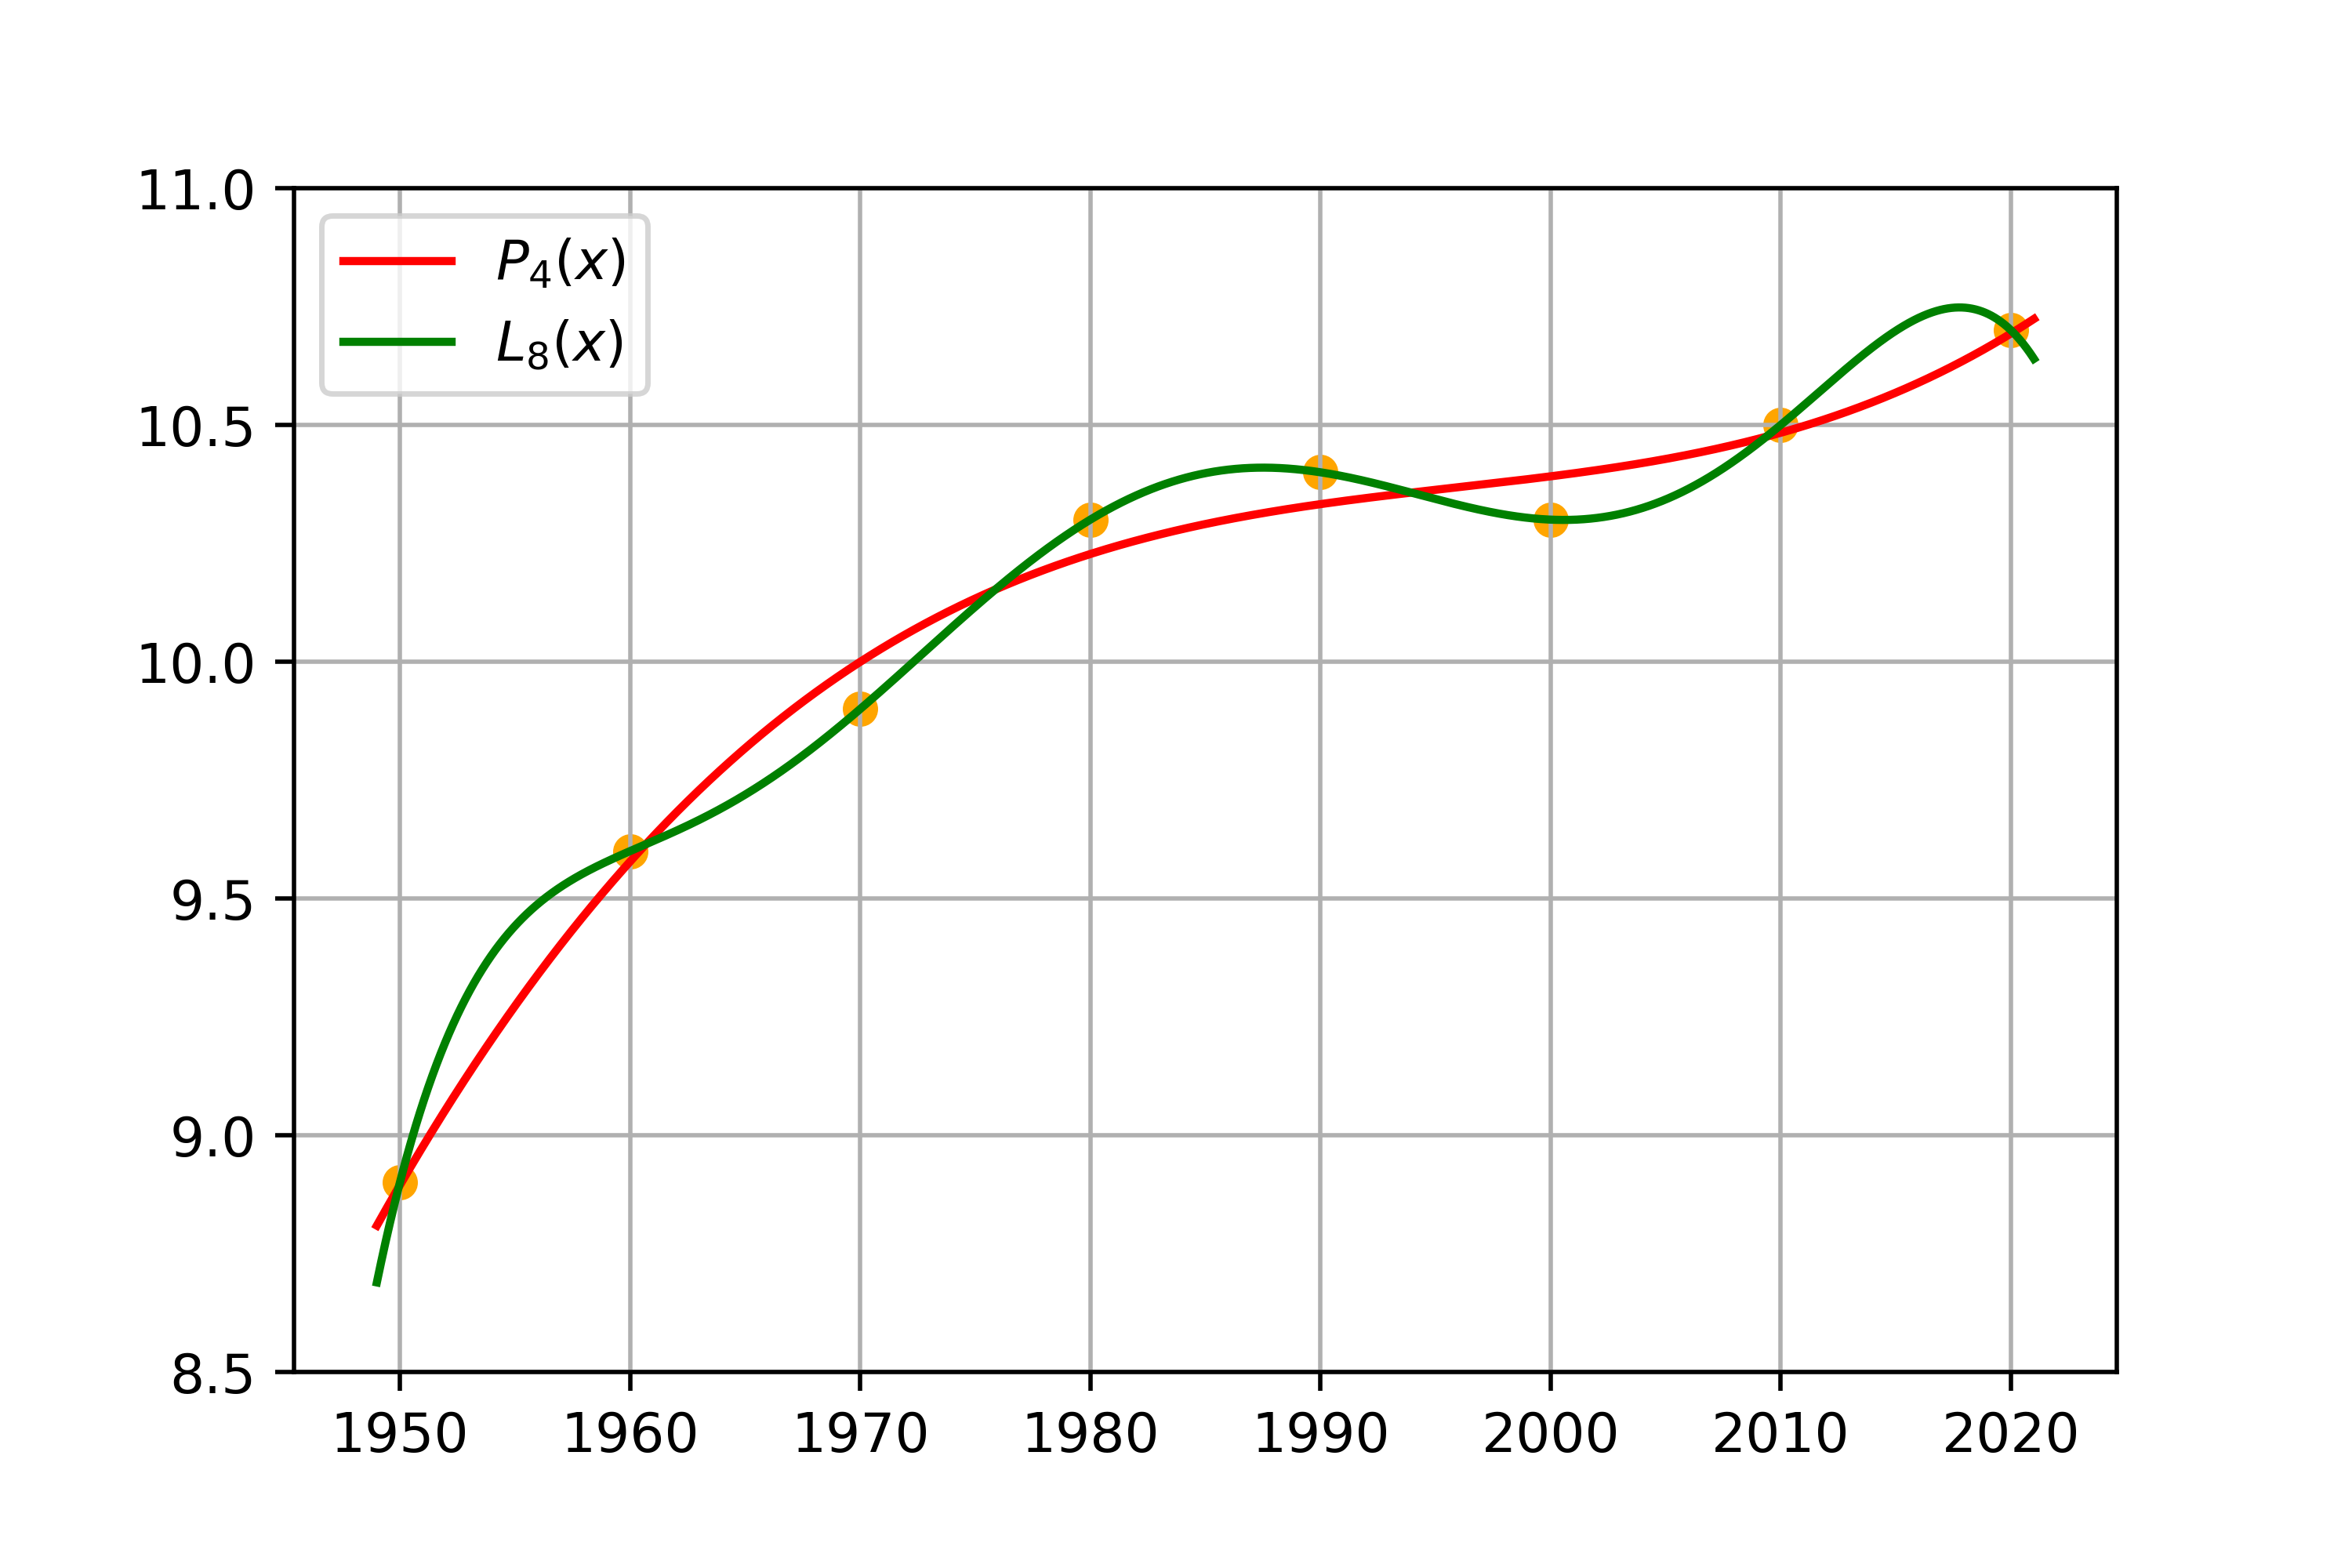
\includegraphics{images/plot_4.1.png}

Вычислив значение численности населения Чехии в 2019 году, и сравнив их с реальным значением получили следующие реузльтаты:

\begin{tabular}{l}
	Метод наименьших квадратов: 10.664 \\
	Интерполяционный многочлен: 10.734 \\
	Реальное значение: 10.669 \\
\end{tabular}

Метод наименьших квадратов дал более точное значение в связи с тем, что такие данные, как численность населения заданы с некоторой погрешностью, из-за чего полином, полученый с помощью МНК, дает более точное представление о динамике численности населения.
\newpage
\subsection*{Код программы}

\begin{lstlisting}
import numpy as np
import matplotlib.pyplot as plt

x = [1950, 1960, 1970, 1980, 1990, 2000, 2010, 2020]
y = [8.9, 9.6, 9.9, 10.3, 10.4, 10.3, 10.5, 10.7]

def Least_Squares(x: list, y: list, m: int):
    s = lambda k: sum([elem**k for elem in x])
    b = lambda k: sum([y[i]*x[i]**k for i in range(len(x))])
    NormalSystem = np.zeros((m+1, m+1))
    for i in range(m+1):
        for j in range(i, m+1):
            temp_coef = s(i + j)
            NormalSystem[i, j] = temp_coef
            NormalSystem[j, i] = temp_coef
    d = np.array([b(i) for i in range(m+1)])
    a = np.linalg.solve(NormalSystem, d)
    return a

def Average_Square_Deviation(Polynom, x, y):
    return (1.0/(len(x)) * sum([(Polynom(x[i]) - y[i])**2 for i in range(len(x))]))**0.5

devs = []
for m in range(1, 6):
    a = Least_Squares(x, y, m)
    Polynom = lambda x: sum([a[i]*x**i for i in range(m+1)])
    devs.append(Average_Square_Deviation(Polynom, x, y))
print(devs)#min(dev) = 0.060136. Polynom degree - 4

a = Least_Squares(x, y, 4)
Polynom = lambda x: sum([a[i]*x**i for i in range(5)])

def Lagrange_Polynom(arg):
    res = 0
    for i in range(len(x)):
        tmp = 1
        for k in range(len(x)):
            if i != k:
                tmp *= (arg - x[k]) * 1.0/(x[i] - x[k])
        res += y[i]*tmp
    return res

print("Least Squares method:", Polynom(2019))
print("Lagrange Polynom:", Lagrange_Polynom(2019))
print("Real value:", 10.669)
\end{lstlisting}
\section*{Задача 4.2}
\subsection*{Постановка задачи}

Дана функция $y = f(x)$. Приблизить функцию методом интерполяции, используя многочлен Лагранжа. Степень $n$ подобрать таким образом, чтобы максимальная величина погрешности на отрезке $[a, b]$ не превышала заданной величины $\varepsilon$. Построить графики многочленов и графики погрешностей. Приблизить функцию методом интерполяции, указанным в индивидуальном варианте (Квадратичный сплайн с дополнительным условием $y'(a) = f'(a)$). Сравнить полученные результаты.
\begin{gather}
	f(x) = x\sin{(2 - x)}, [1, 4] \\
	\varepsilon = 0.001
\end{gather}
	
\subsection*{Теоретический материал}

Так как имеется свобода выбора отрезков разбиения, то имеет смысл выбрать точки таким образом, чтобы погрешность интерполяции была минимальной. Для этого воспользуемся свойством наименее уклонятся от нуля на отрезке $[-1, 1]$ многочленов Чебышева. То есть в качестве узлов интерполяции возьмем нули многочлена Чебышева:

\[
	x_k = \dfrac{a + b}{2} + \dfrac{b - a}{2}\cos{\left(\pi\dfrac{2k + 1}{2n + 2}\right)}, k = 0, 1\dots, n
\]

\textbf{Определение}{
	Сплайном степени $m$ называется функция $S_m(x)$, обладающая следующими свойствами:
	\begin{enumerate}
		\item Функция $S_m(x)$ непрерывна на $[a, b]$ со своими производными.
		\item На каждом отрезке $[x_i, x_{i+1}]$ функция $S_m(x)$ совпадает с некоторым алгебраическим многочленом $P_{m, i}(x)$ степени $m$.
		\item $S_m(x_i) = y_i$, $i = 0, 1\dots n$
	\end{enumerate}
}

\textbf{Определение}{
	Величина $R_n(x) = |f(x) - P_n(x)|$ называется остаточным членом
интерполяции или погрешностью интерполяции.
}

\textbf{Теорема}{
	Пусть функция $f(x)$ дифференцируема $(n+1)$ раз на отрезке $[a, b]$, содержащем узлы интерполяции $x_i$. Тогда для погрешности интерполяции в точке $x \in [a, b]$ справедлива оценка:
	\[
		R_n(x) = |f(x) - P_n(x)| \leq \dfrac{M_{n+1}}{(n+1)!}|\omega_{n+1}(x)|
	\]
	Где $M_{n+1} = max|f^{(n+1)}(x)|$, а $\omega_{n+1}(x) = (x - x_0)\dots(x - x_n)$
}

\subsection*{Решение}

Коэффициенты многочленов сплайна будем искать следующим образом:

\begin{enumerate}
	\item Запишем многочлены в форме $P_i(x) = a_i + b_i(x - x_i) + c_i(x - x_i)(x - x_{i+1})$.
	\item Из условий интерполяции получаем: $a_i = f(x_i)$ а также $a_i + b_i(x_{i+1} - x_i) = a_{i+1} = f(x_{i+1})$, то есть $b_i = \dfrac{a_{i+1} - a_i}{x_{i+1} - x_i}$.
	\item Коэффициенты $c_i$ будем определять из условий непрерывности производной: $P_i'(x_{i+1}) = P_{i+1}'(x_{i+1})$. То есть: $b_i - 2c_ix_i = b_{i+1} - 2x_{i+2}c_{i+1}$. В конечном итоге получаем следующую формулу для $c_{i+1}$: $c_{i+1} = \dfrac{b_{i+1} - b_i}{2x_{i+2}} + \dfrac{x_i}{x_{i+2}}c_i$.
\end{enumerate}
\newpage
\subsection*{Анализ результатов}
Приведем графики исходной функции $f(x)$, интерполяционного многочлена Лагранжа $L(x)$ и квадратичного сплайна $P(x)$(так как функция приближалась с точностью  $\varepsilon=10^{-3}$, то при данном масштабе различия между ними незаметны):

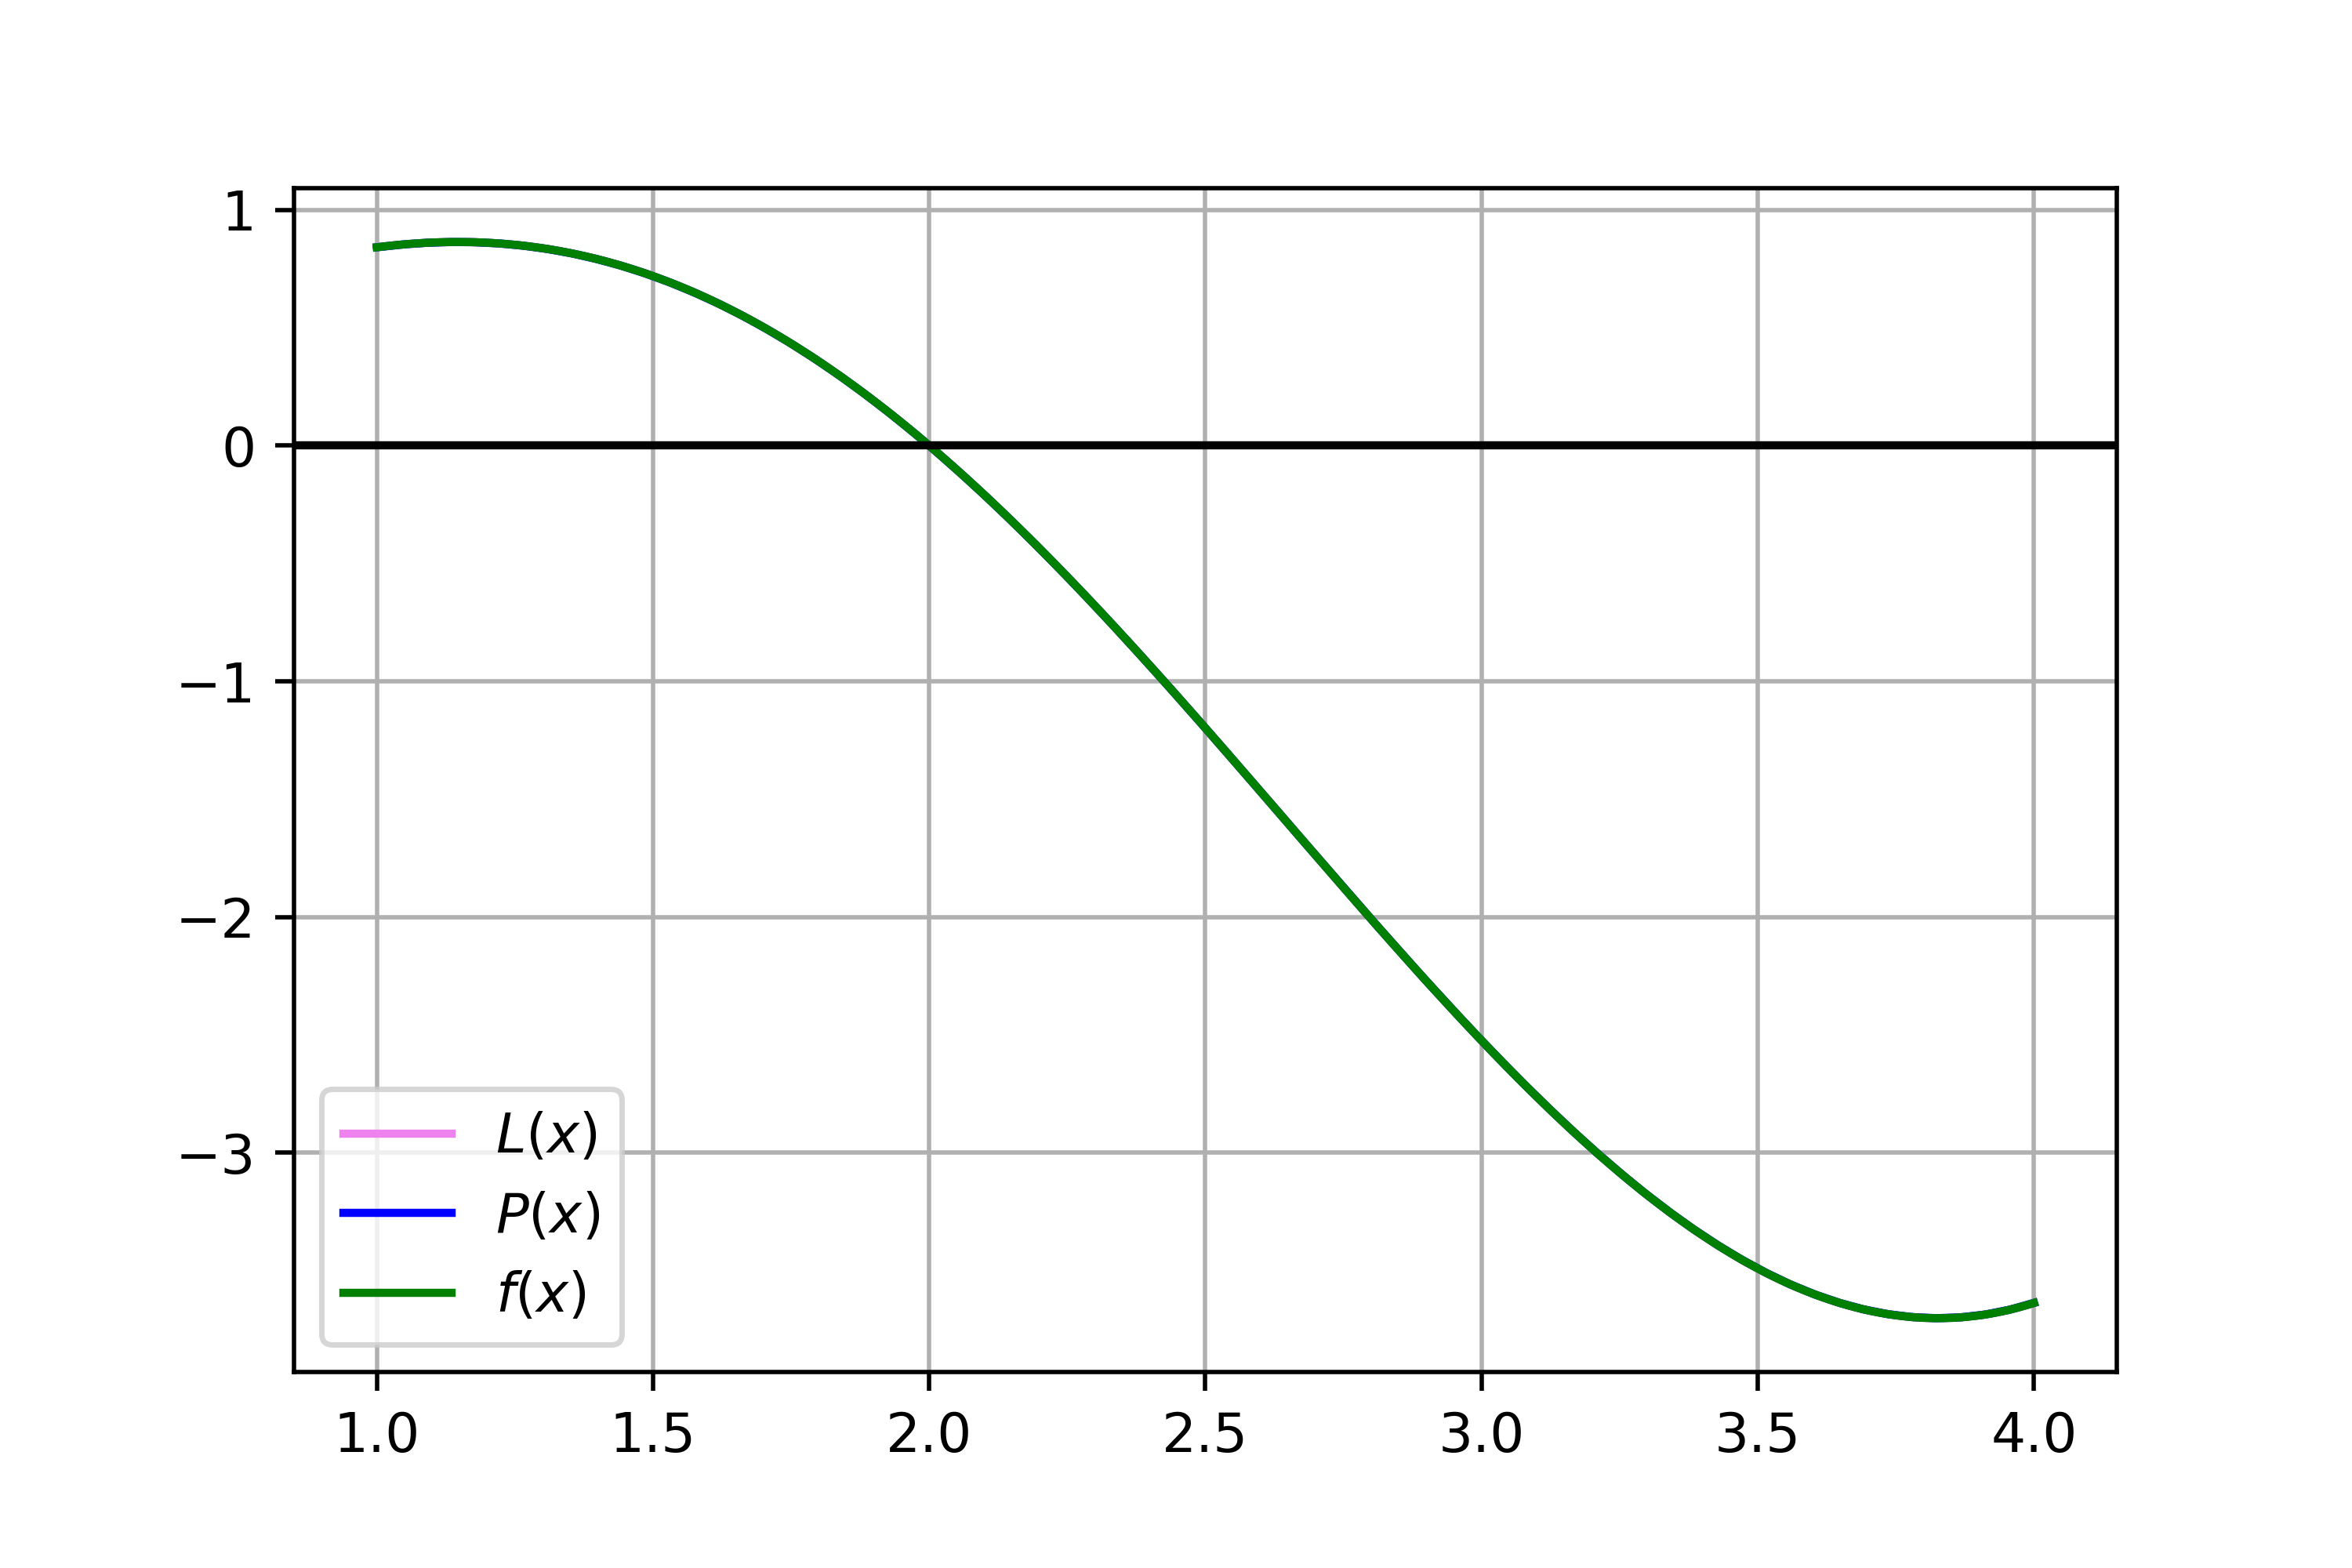
\includegraphics[height=6cm]{images/plot_4.2_all_inter.png}

Анализ графиков погрешности показал, что выбор узлов интерполяции согласованно с нулями многочленов Чебышева дает значительный прирост в точности для глобальной интерполяции функции на отрезке с помощью многочлена 6-ой степени (7 узлов) в форме Лагранжа(см. рис.) - в случае равномерной сетки максимальная погрешность на отрезке чуть меньше $10^{-3}$, а с помощью узлов Чебышева максимальная погрешность немногим больше $0.25 \cdot 10^{-3}$, то есть в 3-4 раза меньше.

\begin{figure}[h!]
	\centering                                                                                            
	\begin{minipage}{0.45\textwidth}
	        \centering
	        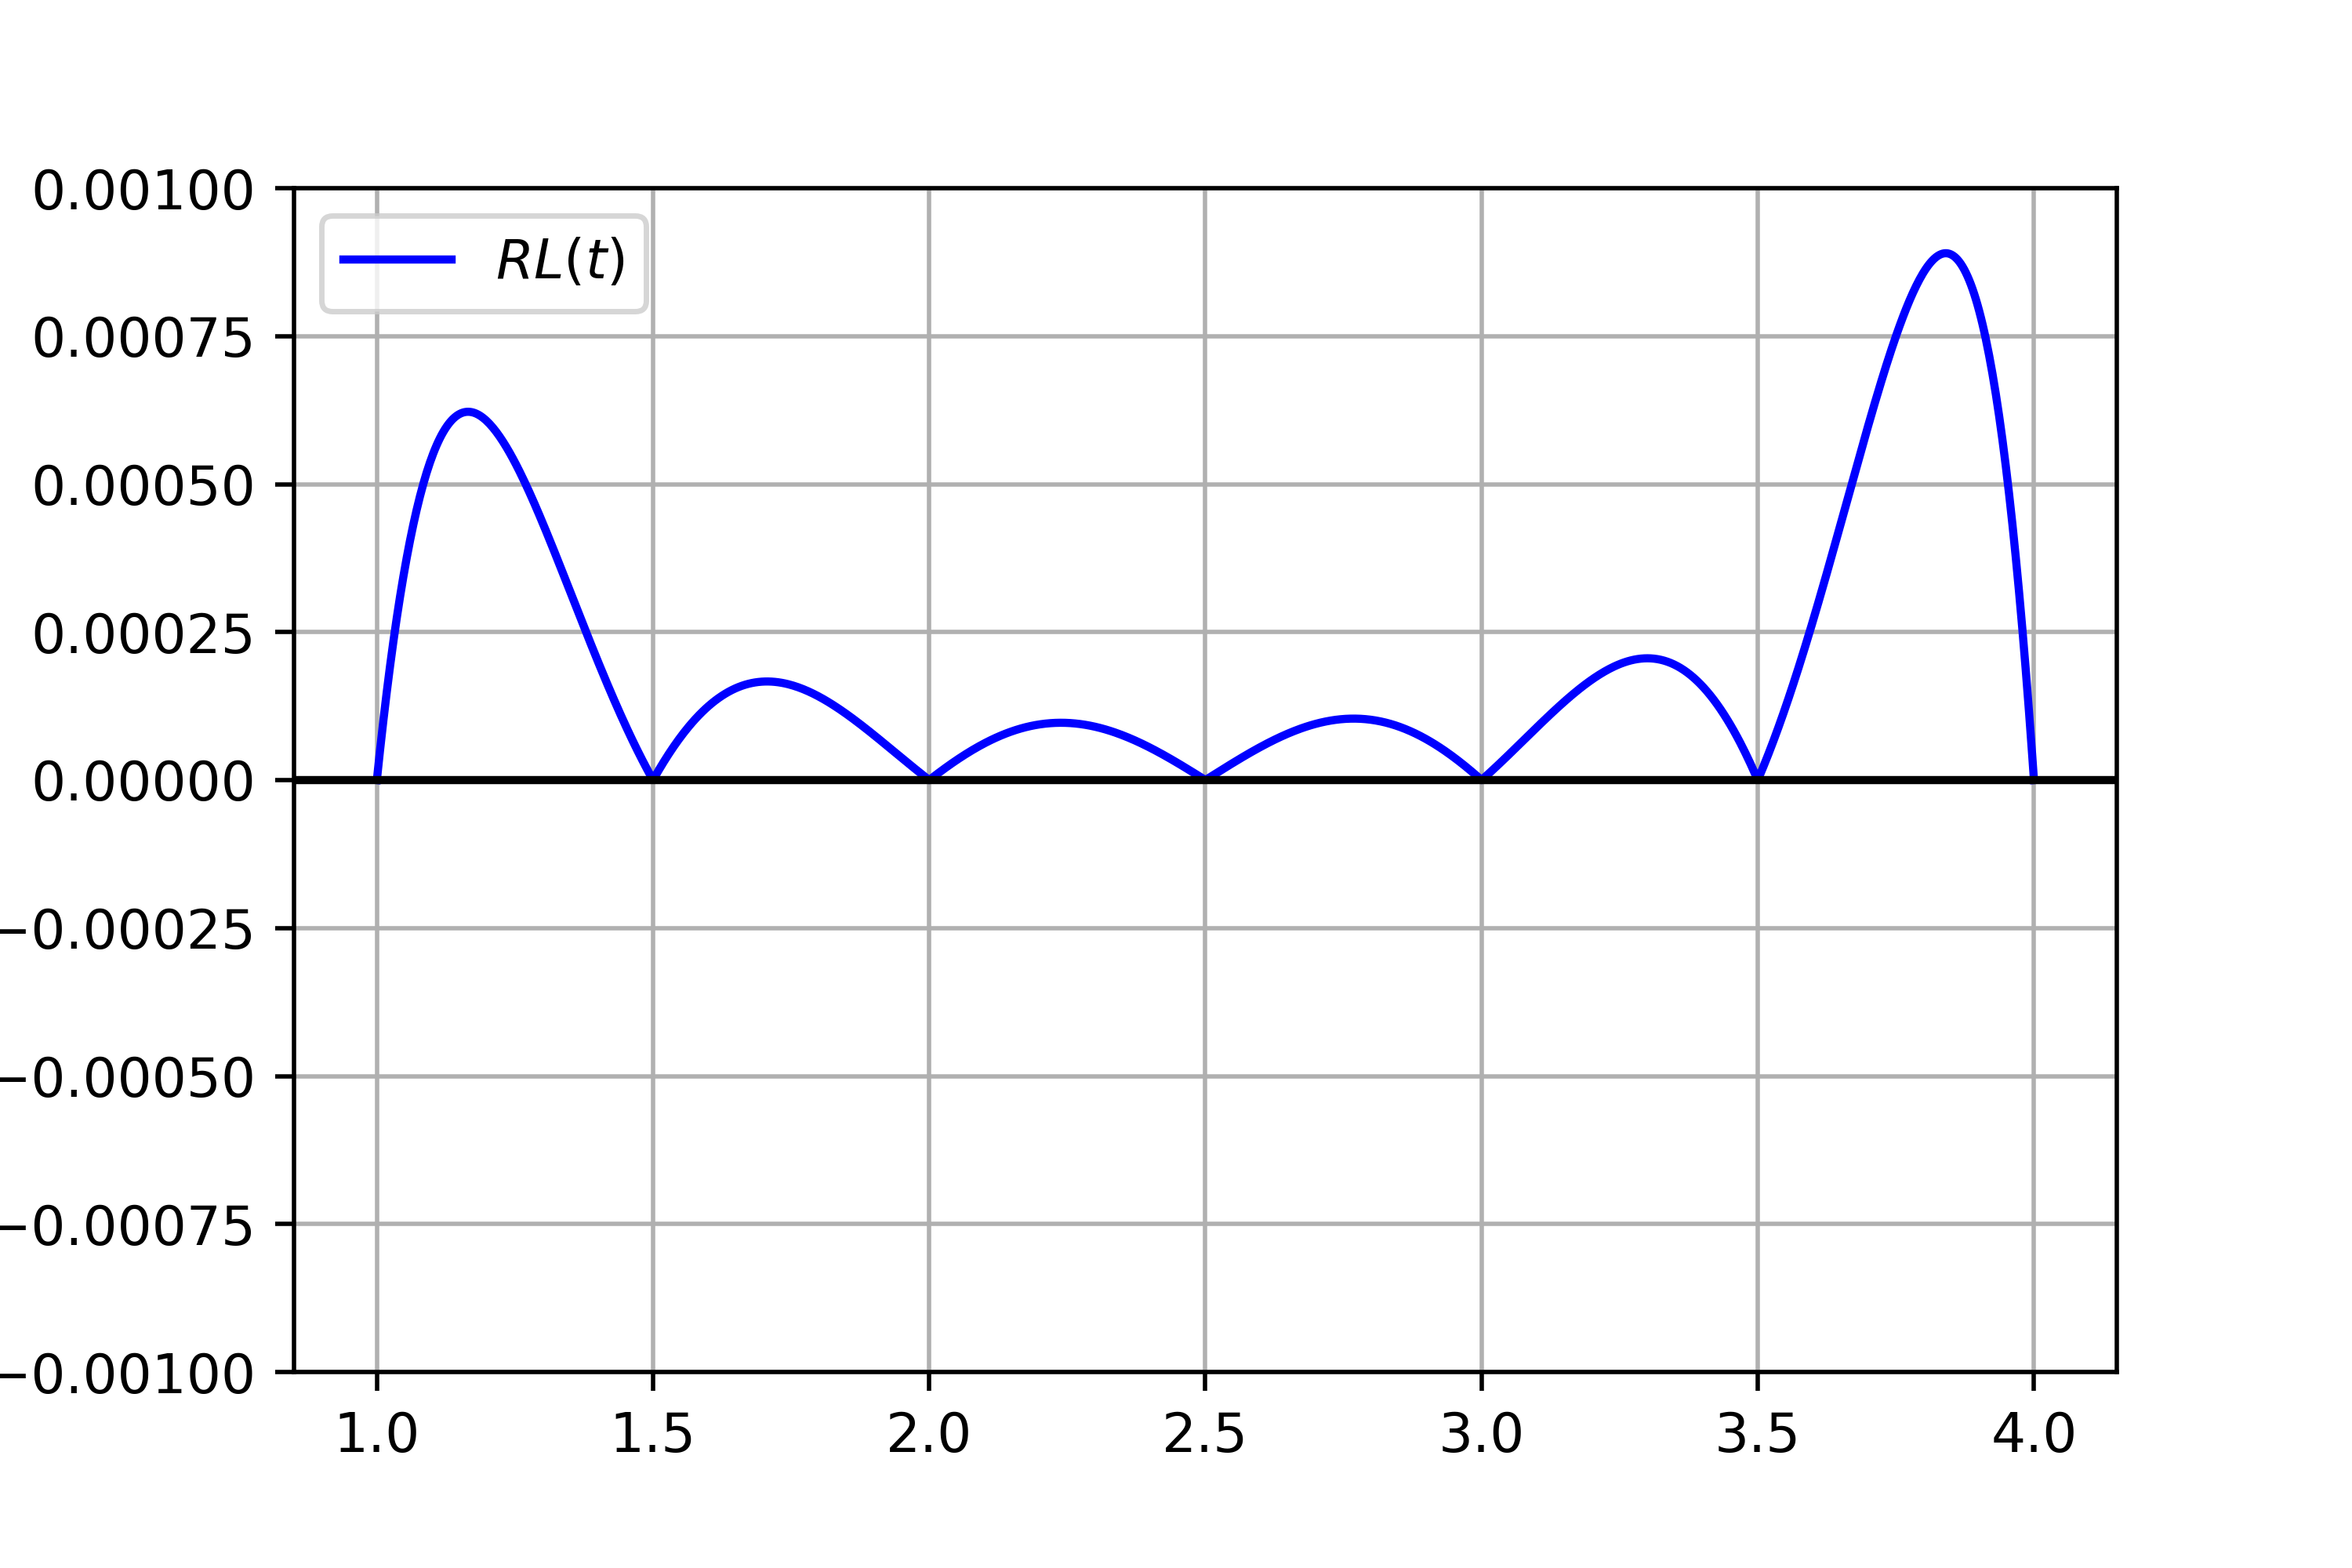
\includegraphics[width=8cm]{images/plot_4.2_err_Lagrange_equal.png} % первое изображение
	        \caption{Погрешность глобальной интерполяции при равномерном выборе узлов интерполяции}
	\end{minipage}\hfill
	\begin{minipage}{0.45\textwidth}
		\centering
		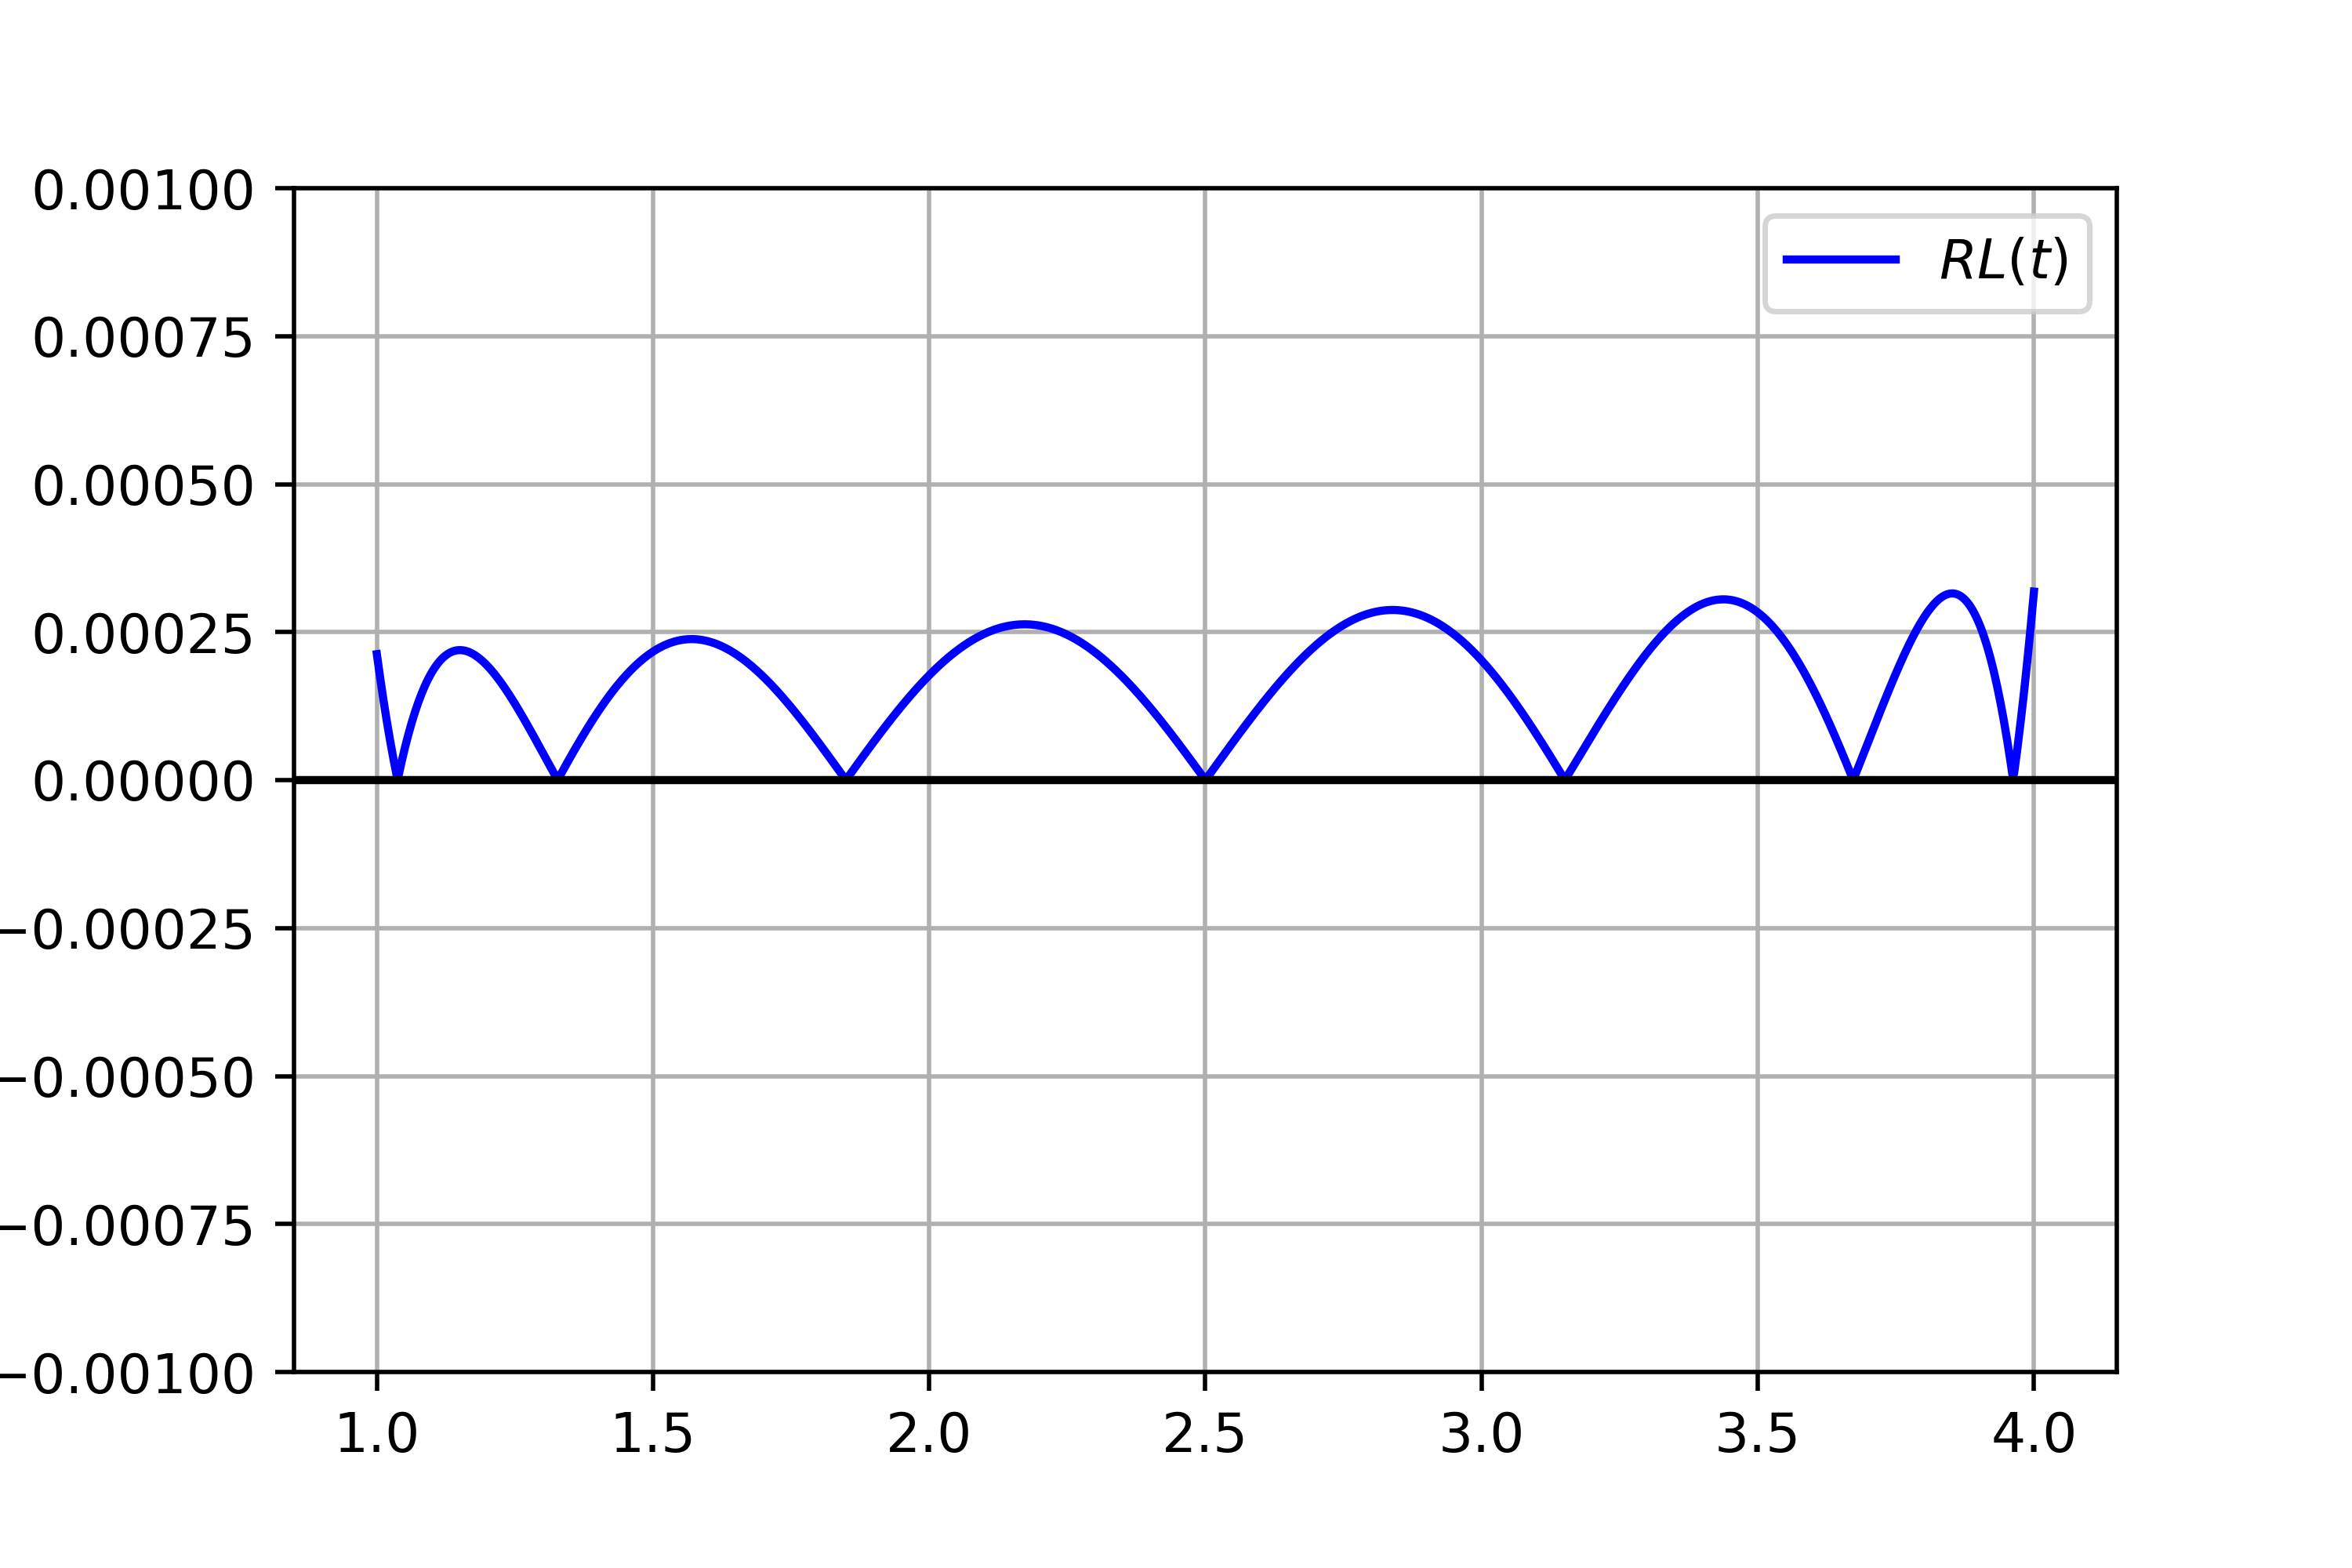
\includegraphics[width=8cm]{images/plot_4.2_err_Lagrange_Chebyschev.png} % второе изображение
		\caption{Погрешность глобальной интерполяции при выборе "Чебышевских" узлов}
	\end{minipage}
\end{figure}

Однако при приближении функции с помощью квадратичного сплайна наблюдается обратная ситуация - погрешность больше, если выбирать узлы соответственно нулям Чебышева (в обоих случаях $n = 69$). Соответственно, на первом графике данного раздела изображен более точный сплайн.

\begin{figure}[h!]
	\centering                                                                                            
	\begin{minipage}{0.45\textwidth}
	        \centering
	        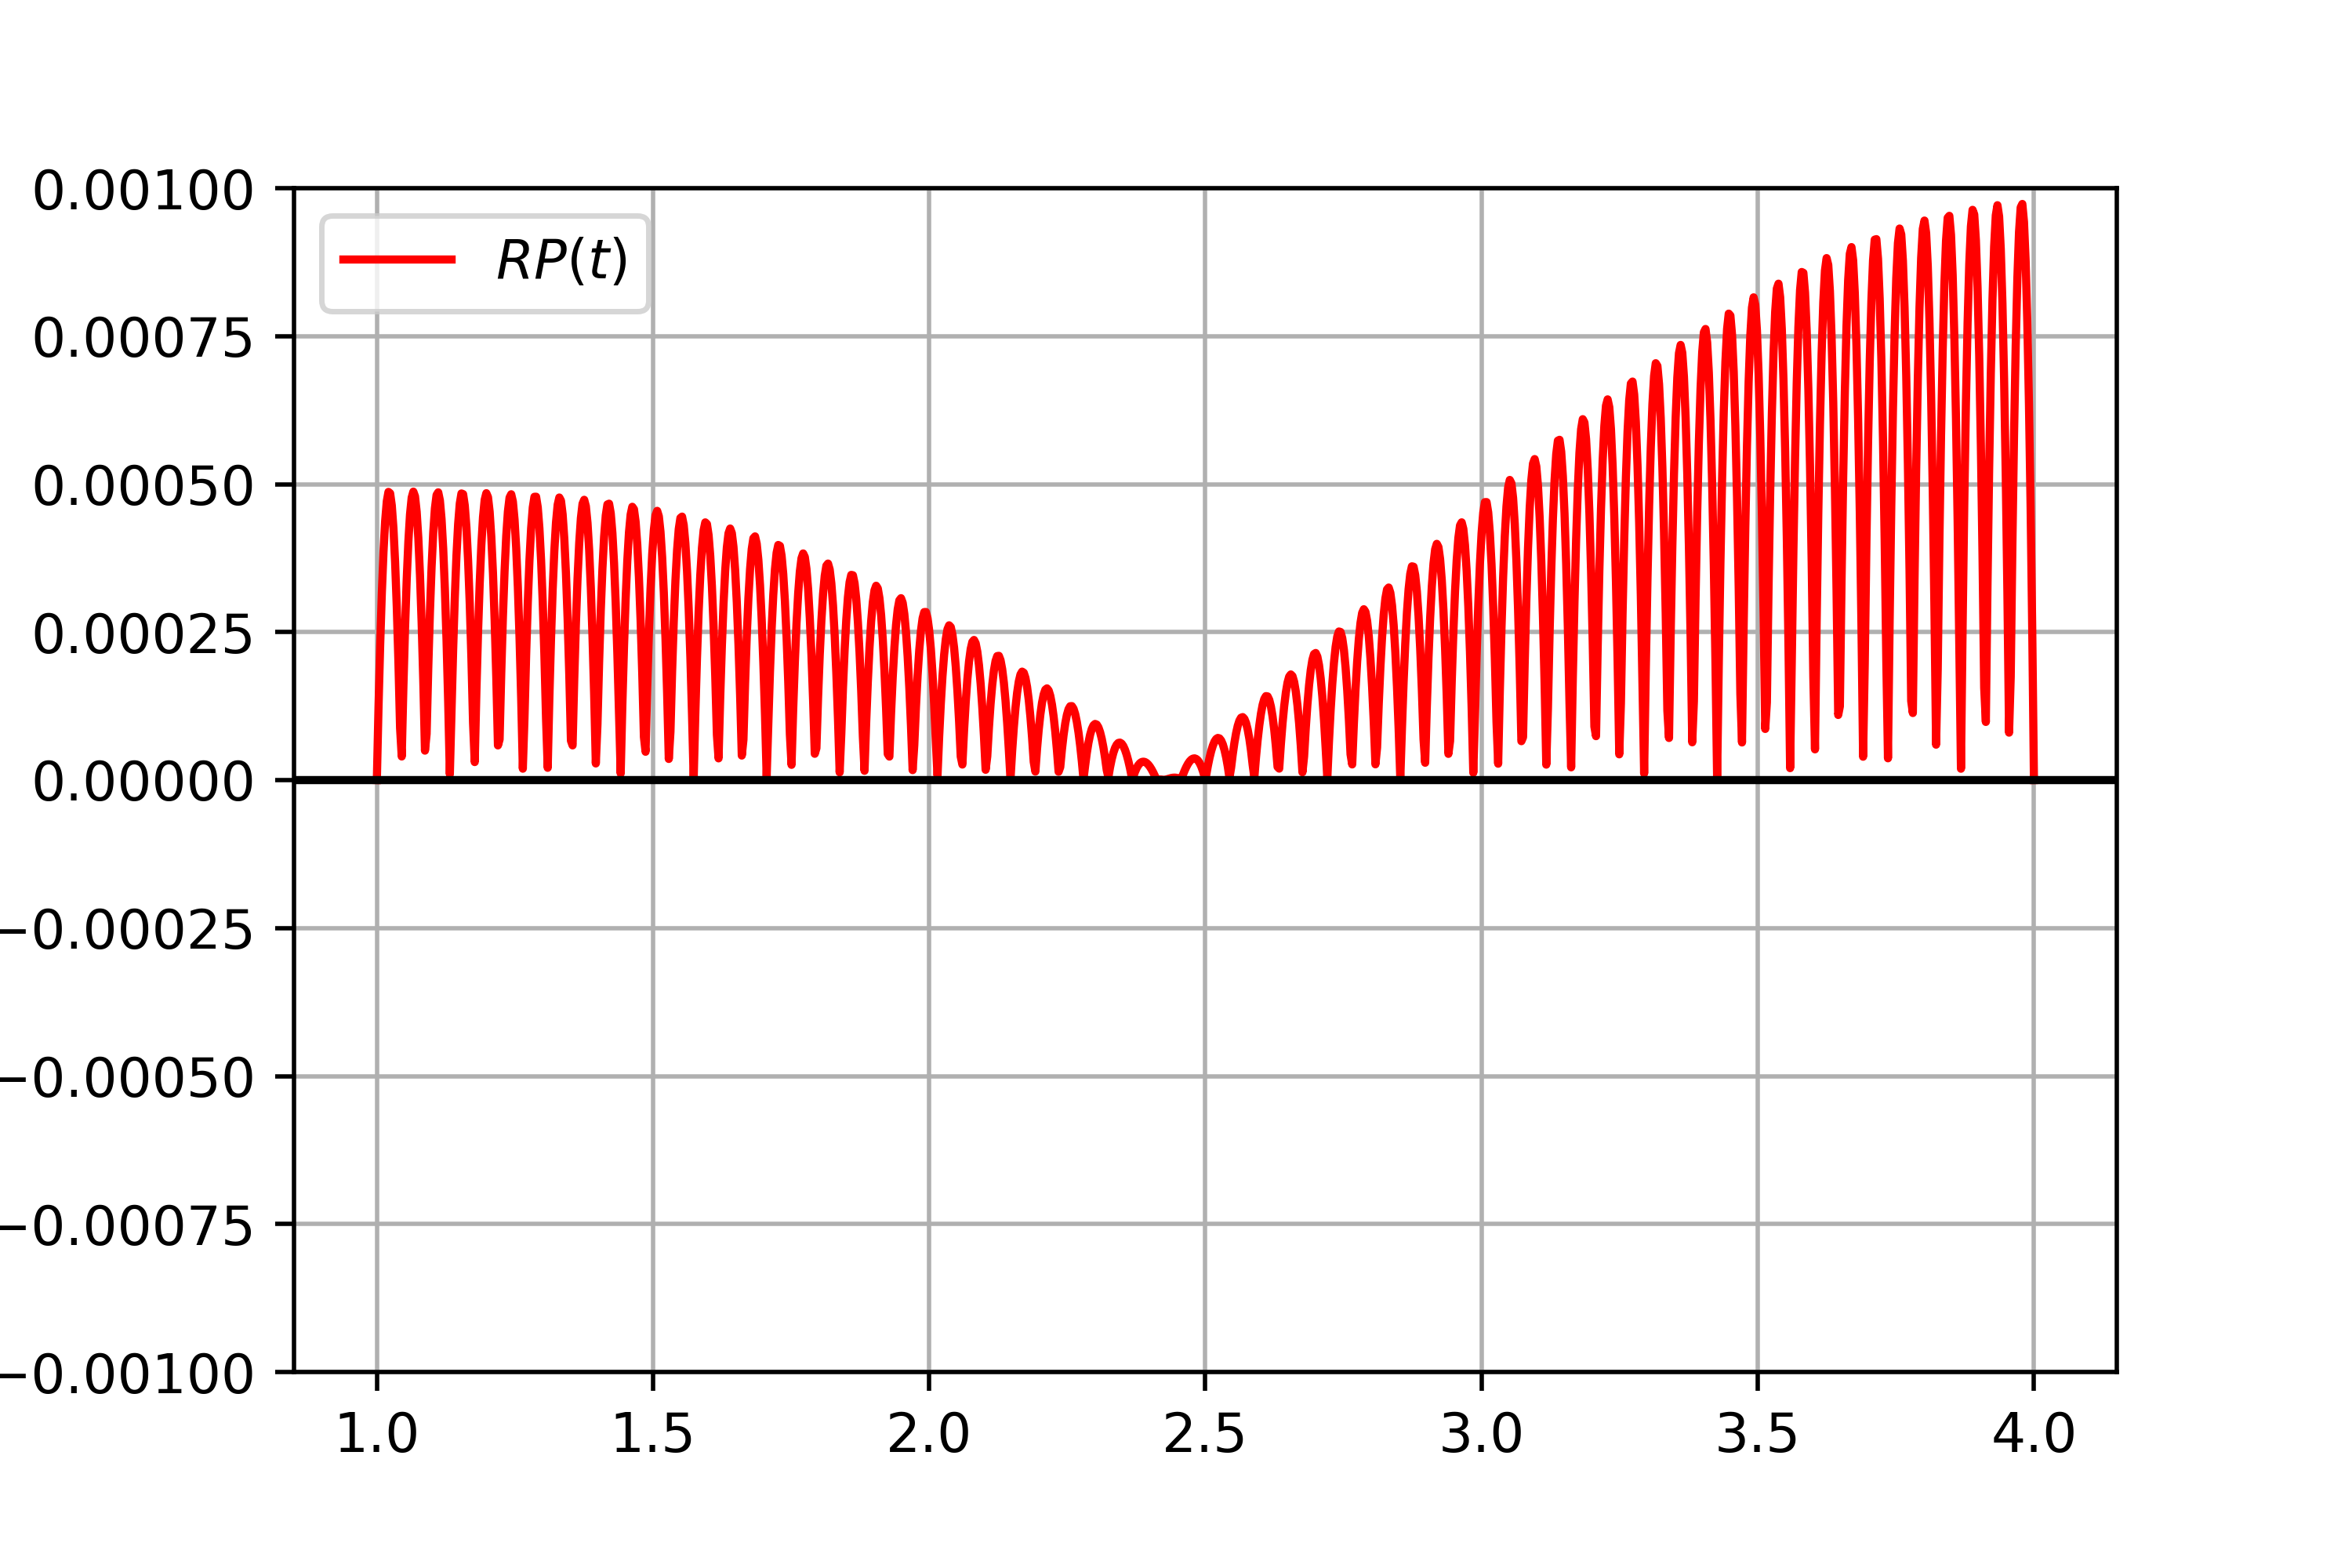
\includegraphics[width=8cm]{images/plot_4.2_err_Spline_equal.png} % первое изображение
	        \caption{Равномерная сетка}
	\end{minipage}\hfill
	\begin{minipage}{0.45\textwidth}
		\centering
		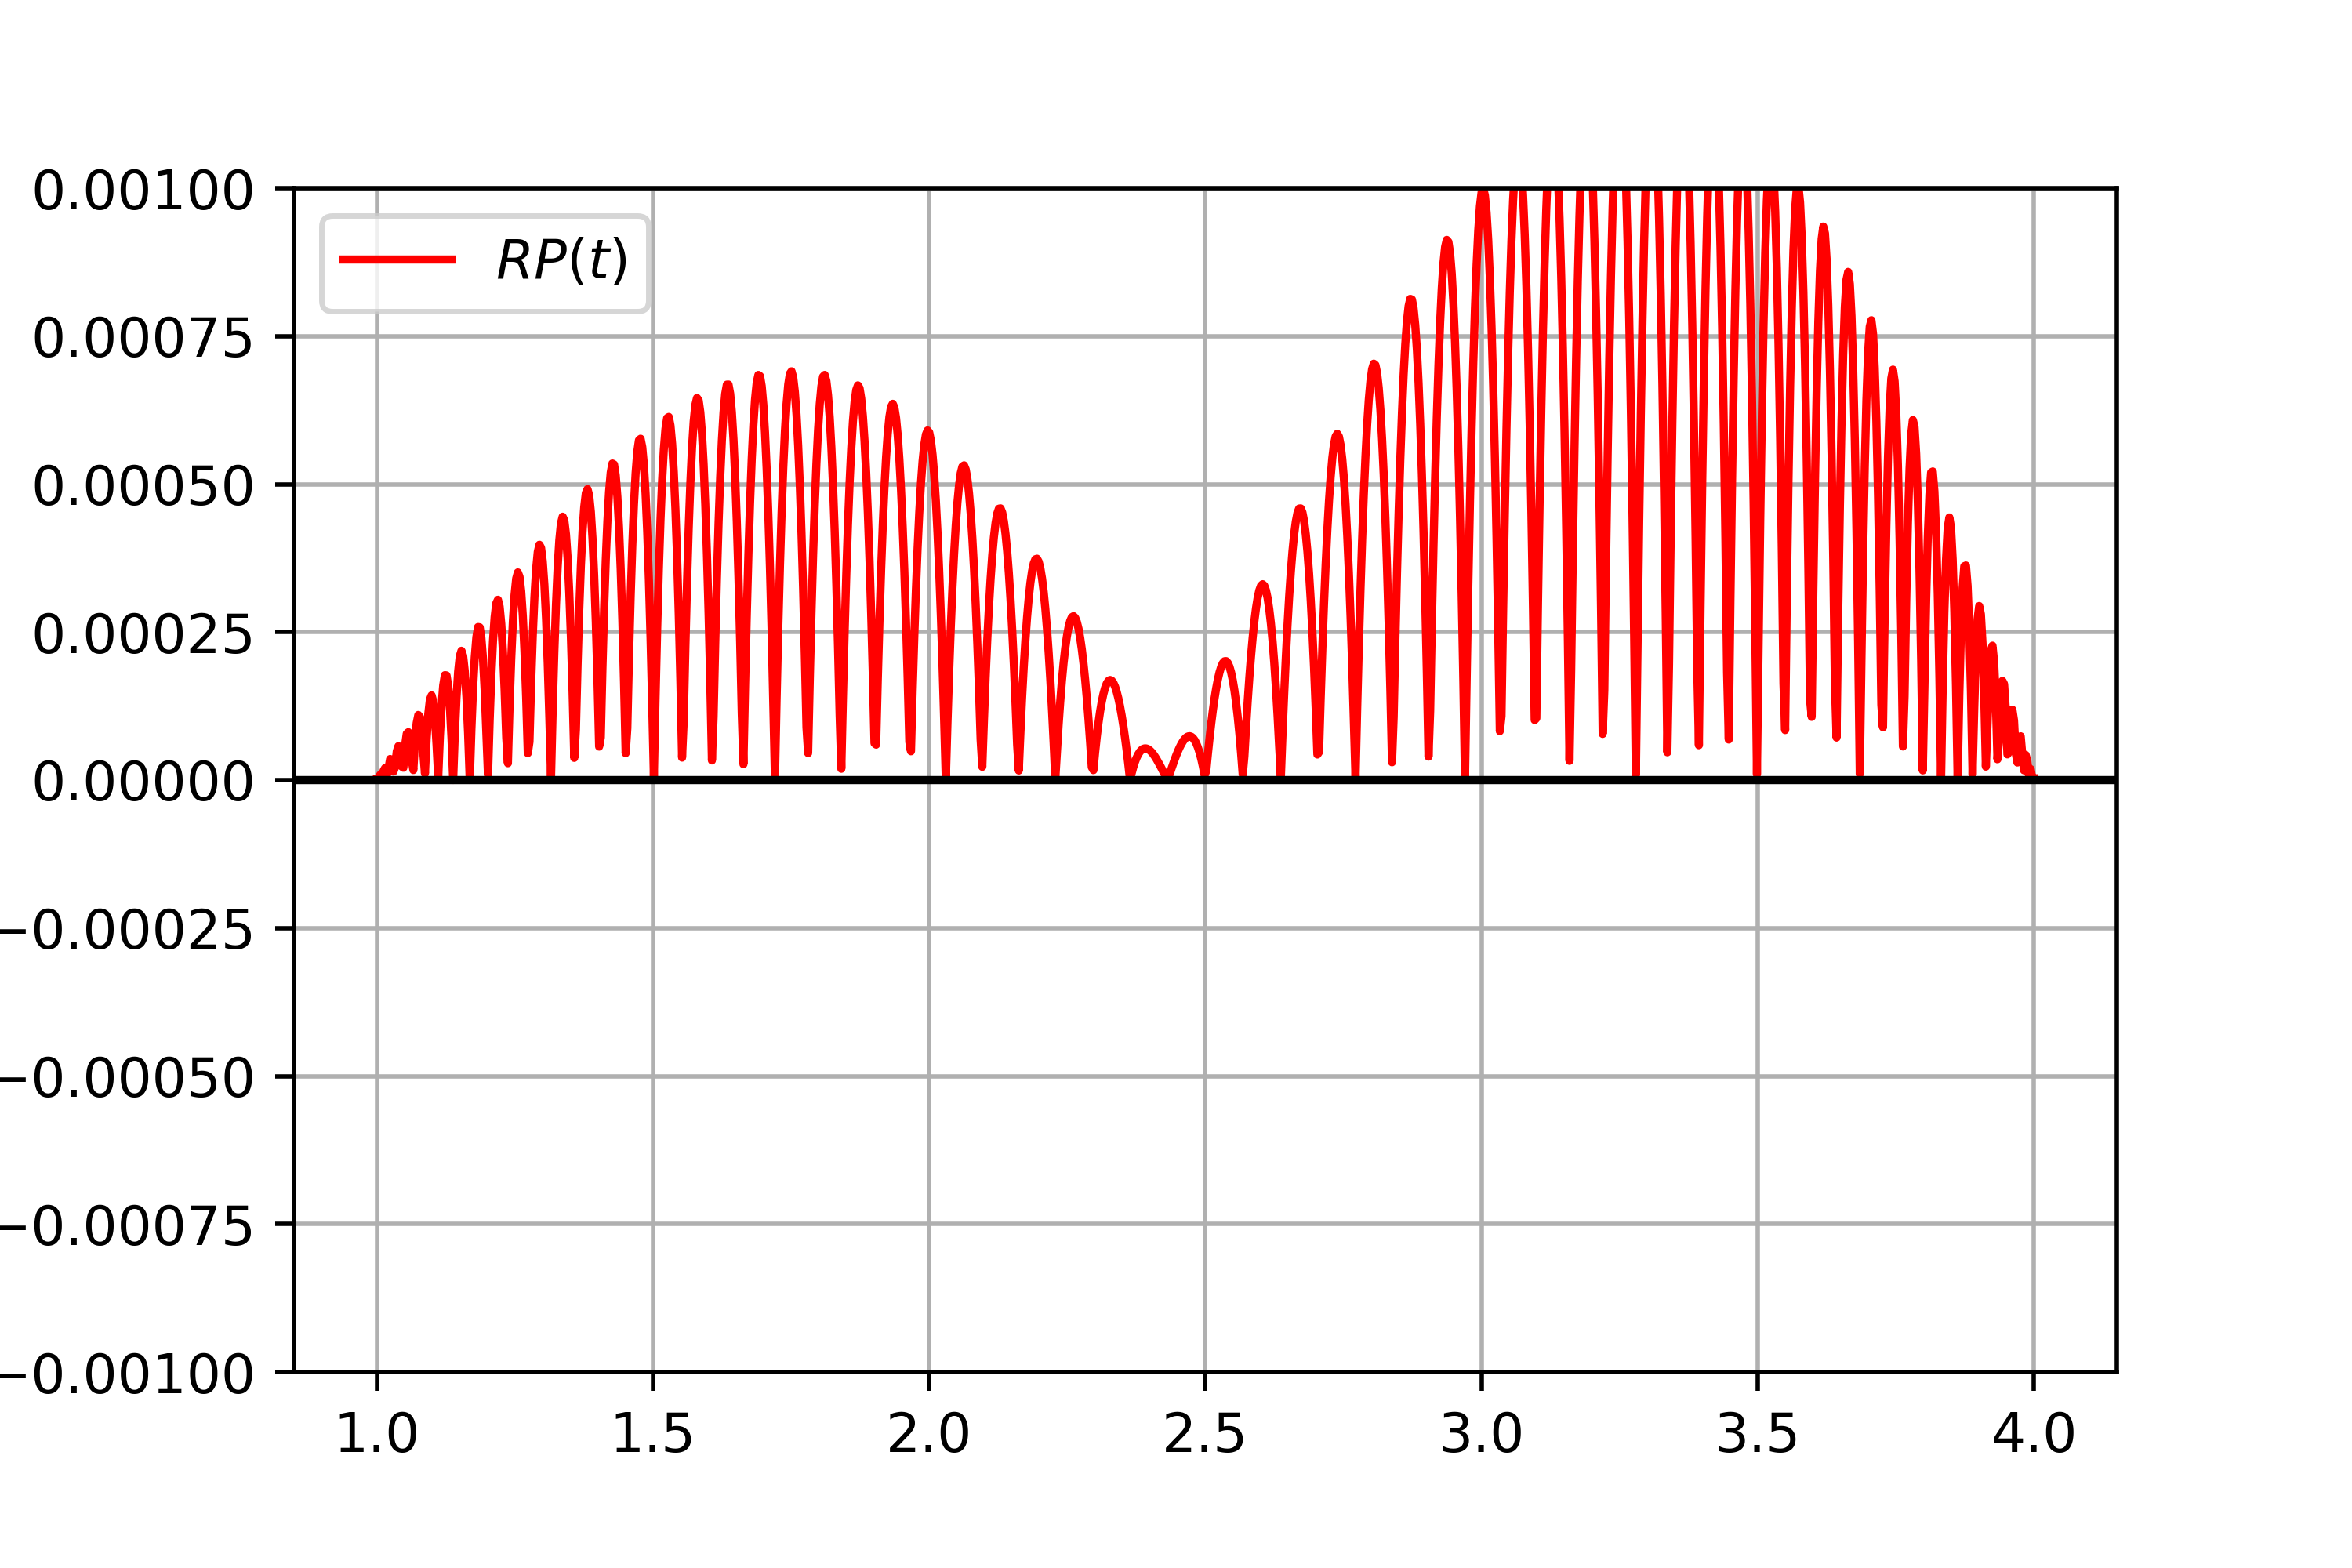
\includegraphics[width=8cm]{images/plot_4.2_err_Spline_Chebyschev.png} % второе изображение
		\caption{Чебышевские узлы}
	\end{minipage}
\end{figure}

Стоит отметить, что на обоих графиках явно выделяется точка, где обе погрешности минимальные - это точка перегиба, то есть где вторая производная равна нулю.

\subsection*{Код программы}
\begin{lstlisting}
import numpy as np
import matplotlib.pyplot as plt
from collections import namedtuple

def f(x: np.float64) -> np.float64:
    #return 1.0 / (1 + 25*x**2)
    return x*np.sin(2 - x)

def equal_partition(a: np.float64, b: np.float64, n: int) -> np.ndarray:
    return np.linspace(a, b, n)

def Chebyschev_partition(a: np.float64, b: np.float64, n: int) -> np.ndarray:
    n -= 1
    get_x = lambda k: 0.5*(a + b) + 0.5*(b - a) * np.cos(np.pi * (2*k + 1)/(2*n + 2))
    x = [get_x(k) for k in range(n, -1, -1)]
    partition = np.array(x)
    return partition

Polynom = namedtuple("Polynom", ["a", "b", "c", "x0", "x1"])
def make_spline(x: np.ndarray, y: np.ndarray, dfa: np.float64):
    spline = []
    n = len(x) - 1
    a, b, c = [0]*n, [0]*n, [0]*n
    for i in range(n):
        a[i] = y[i]
        b[i] = (y[i+1] - y[i]) / (x[i+1] - x[i])
    c[0] = (dfa - b[0])/(2*x[1])
    spline.append(Polynom(a[0], b[0], c[0], x[0], x[1]))
    for i in range(1, n):
        c[i] = (b[i] - b[i-1])/(2 * x[i+1]) + x[i-1]/x[i+1] * c[i-1]
        spline.append(Polynom(a[i], b[i], c[i], x[i], x[i+1]))
    return spline

a, b = 1, 4
n_dots = 69
x = equal_partition(a, b, n_dots) #100 0.005909864879679992
#x = Chebyschev_partition(a, b, n_dots) #100 0.007819083547945267
y = np.array([f(i) for i in x])
df1 = np.sin(1) - np.cos(1)
spline = make_spline(x, y, df1)

def Spline(arg: np.float64):
    n = len(spline)    
    if arg <= spline[0].x1:
        s = spline[0]
    elif arg >= spline[n - 1].x0:
        s = spline[n - 1]
    else:
        i, j = 0, n - 1
        while i + 1 < j:
            k = i + (j - i) // 2
            if arg <= spline[k].x0: j = k
            else: i = k
        s = spline[i]
    return s.a + s.b*(arg - s.x0) + s.c*(arg - s.x0)*(arg - s.x1)

x = Chebyschev_partition(a, b, 7)
y = np.array([f(i) for i in x])
def Lagrange_Polynom(arg):
    res = 0
    for i in range(len(x)):
        tmp = 1
        for k in range(len(x)):
            if i != k:
                tmp *= (arg - x[k])* 1.0/(x[i] - x[k])
        res += y[i]*tmp
    return res
\end{lstlisting}

\section*{Задача 4.3}
\subsection*{Постановка задачи}
Задана функция $f(x) = e^{2x} - 1$, определенная на отрезке $[-1, 1]$. Требуется разложить функцию в рял Тейлора в окрестности нуля с точностью $\varepsilon$ и произвести экономизацию полученного степенного ряда.

\subsection*{Теоретический материал}
Суть метода экономизации степенного ряда заключается в следующем:

\begin{enumerate}
	\item Берем отрезок ряда Тейлора $P_m(x) = \sum\limits_{k = 0}^m a_kx_k$, аппроксимирующий функцию $f(x)$ с точностью $\varepsilon_0 < \varepsilon$.
	\item Выражая $x^m$ с помощью многочлена Чебышева, заменяем $x^m$ в разложении Тейлора на $-2^{1 - m}(b_0 + b_1x + \dots + b_{m - 1} x^{m-1}) + 2^{1 - m}T_m(x)$ до тех пор, пока величина погрешности не превысит заданного значения.
\end{enumerate}

\subsection*{Решение}
Запишем разложение функции $f(x) = e^{2x} - 1$ в ряд Тейлора:
\[
	f(x) = e^{2x} - 1 = \sum\limits_{n = 1}^\infty \dfrac{2^nx^n}{n!}
\]

\begin{enumerate}
	\item Определим функцию, вычисляющую $a_k$ коэффициент разложения ряда Тейлора и функцию, вычисляющую значение ряда в данной точке.
	\item Найдем число $n$ - длину ряда, вычисляющего значение функции на заданном отрезке с необходимой точностью с помощью оценки сверху для остаточного члена разложения в форме Лагранжа: $max(r_n(x)) = \dfrac{f^{(n+1)}(\xi)x^{n+1}}{(n+1)!} \leq \dfrac{2^{n+1}}{(n+1)!} \leq \varepsilon$.
	\item Для первого слагаемого замены при экономизации воспользуемся готовыми формулами.
	\item Параллельно будем строить графики получившихся замен до тех пор, пока не достигнем максимально допустимой точности.
\end{enumerate}

Для реализации процесса экономизации степенного ряда воспользуемся встроенными средствами библиотеки NumPy для работы с многочленами - numpy.polynomial.

\newpage
\subsection*{Анализ результатов}
Для того, чтобы достичь необходимой точности ($\varepsilon = 10^{-8}$) необходимо взять 16 членов ряда Тейлора.

Проводя экономизацию ряда с 15 до 11 степени удалось сохранить необходимую точность:
\begin{figure}[h!]
	\centering                                                                                            
	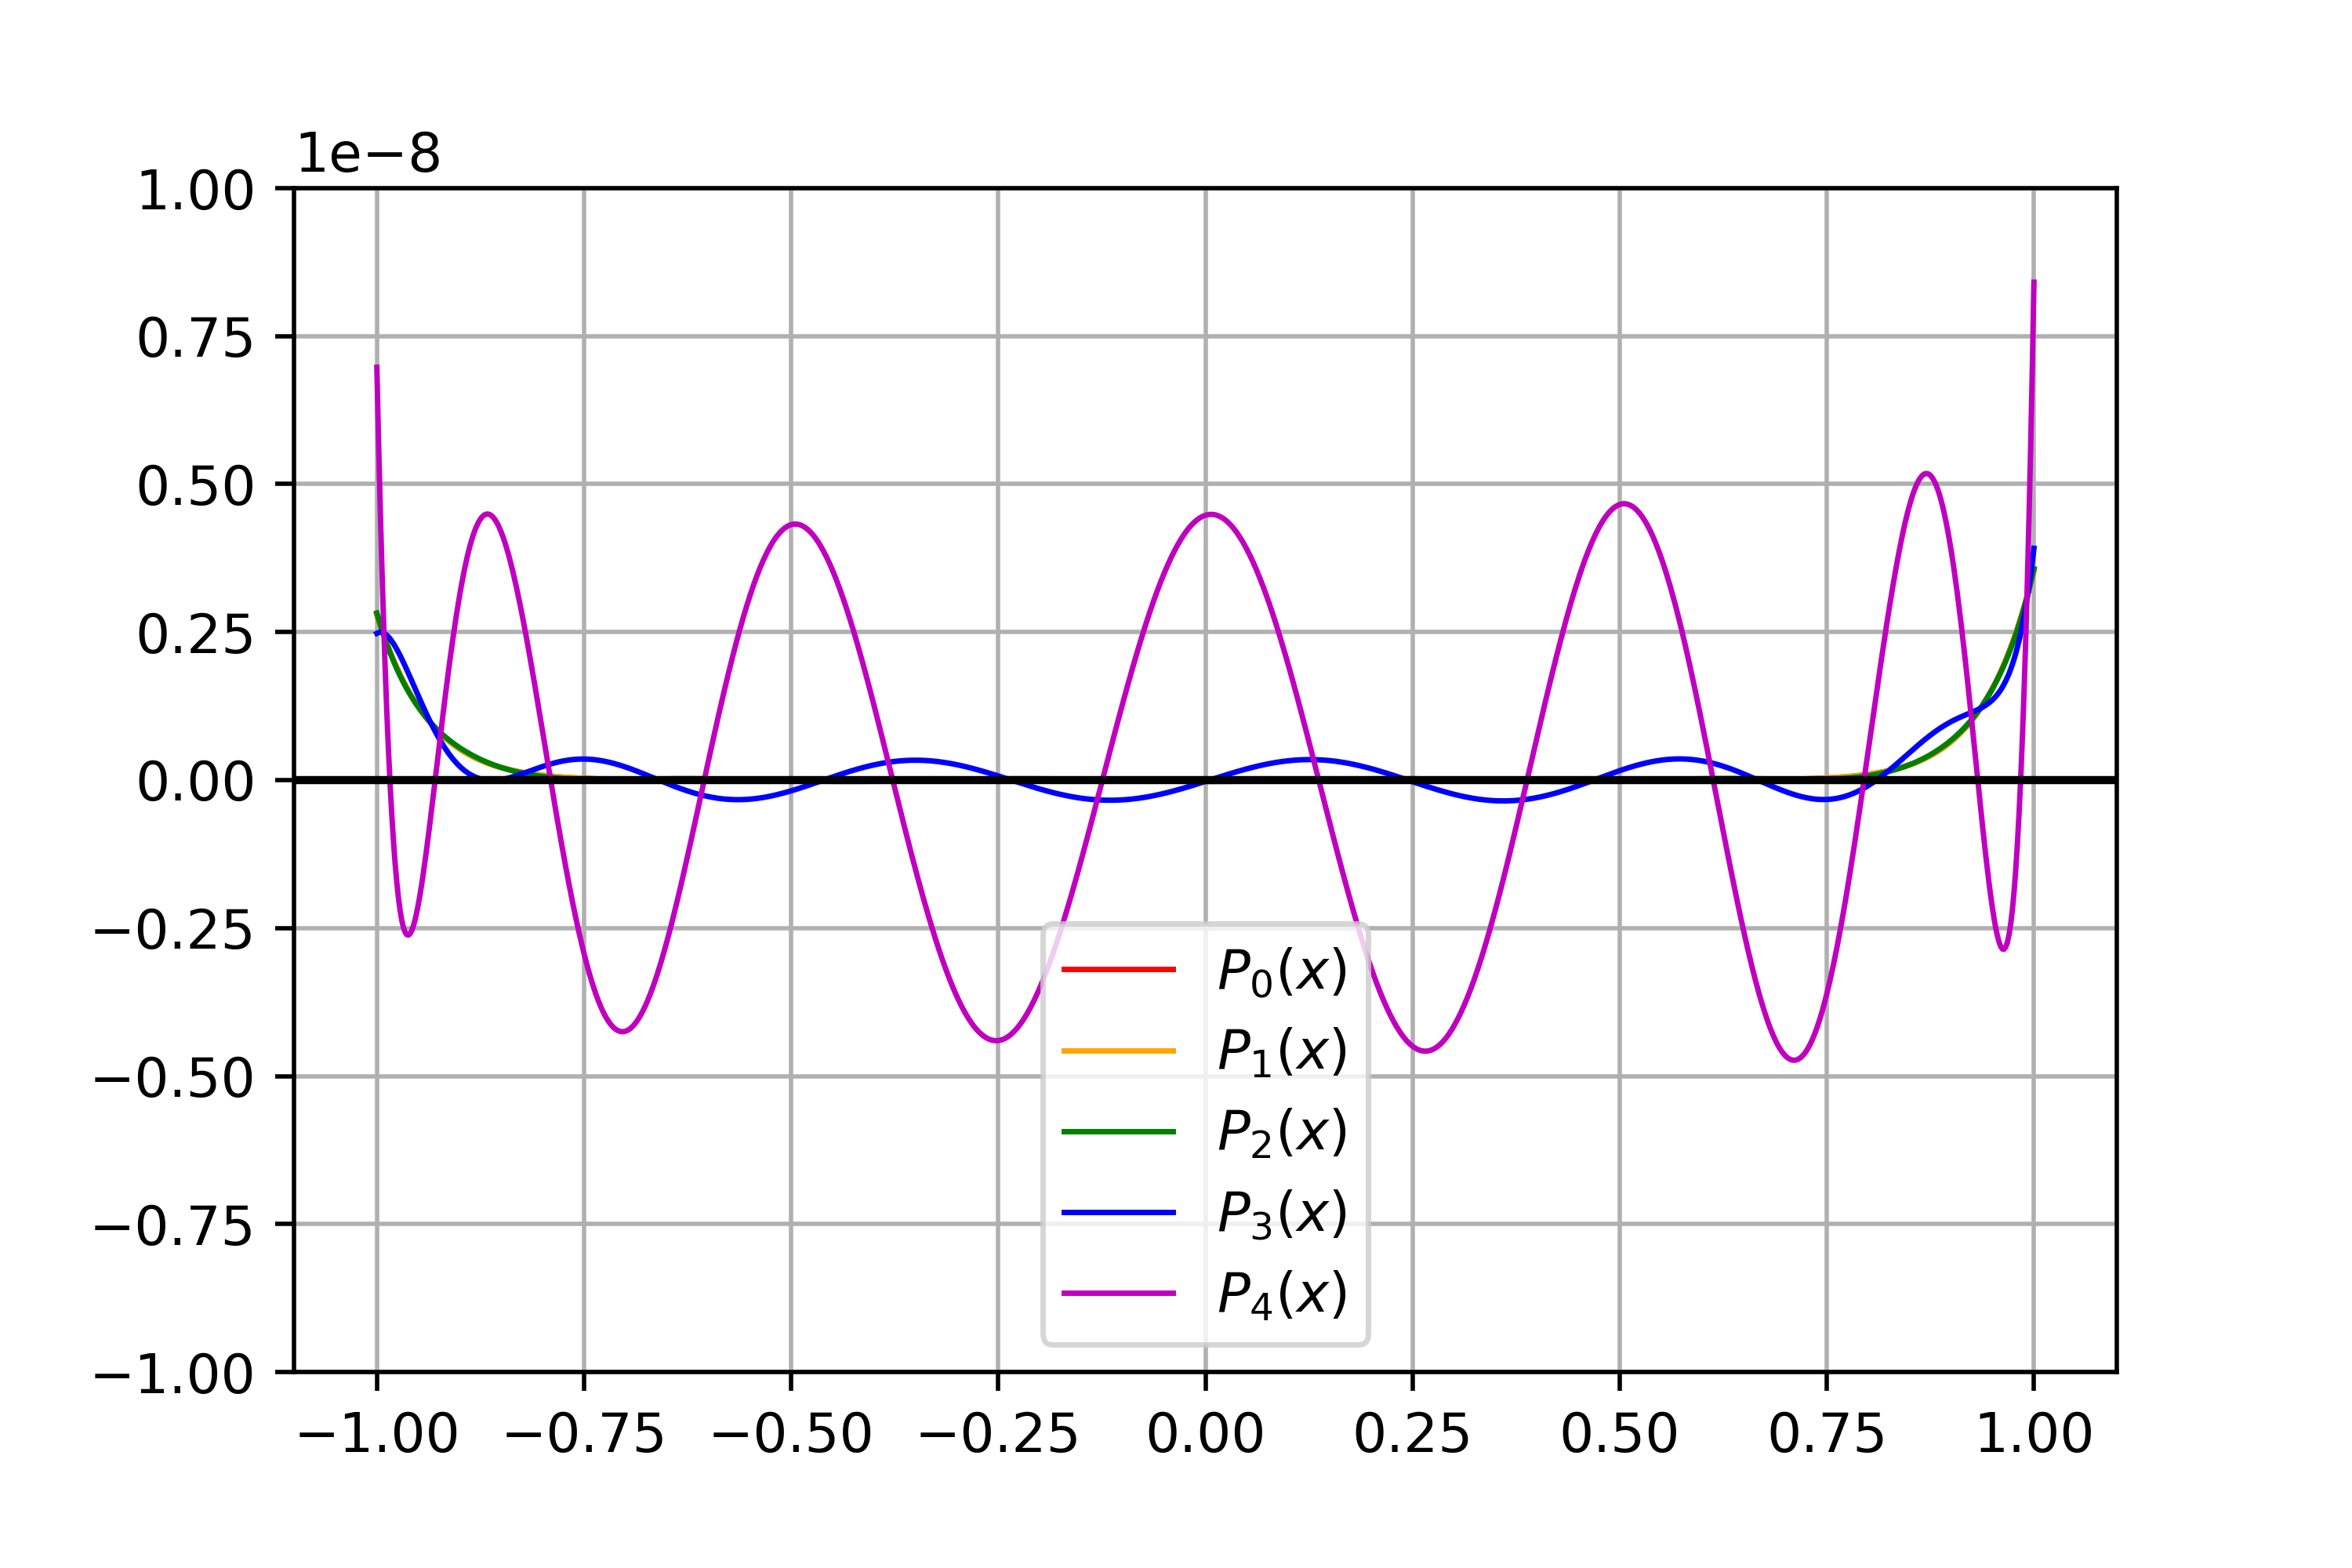
\includegraphics[height=8cm]{images/plot_4.3_err.png}
	\caption{Погрешность ряда на каждом этапе экономизации. $P_0(x)$ - до экономизации. $P_4(x)$  - после завершения процесса}
\end{figure}

График ряда после экономизации:

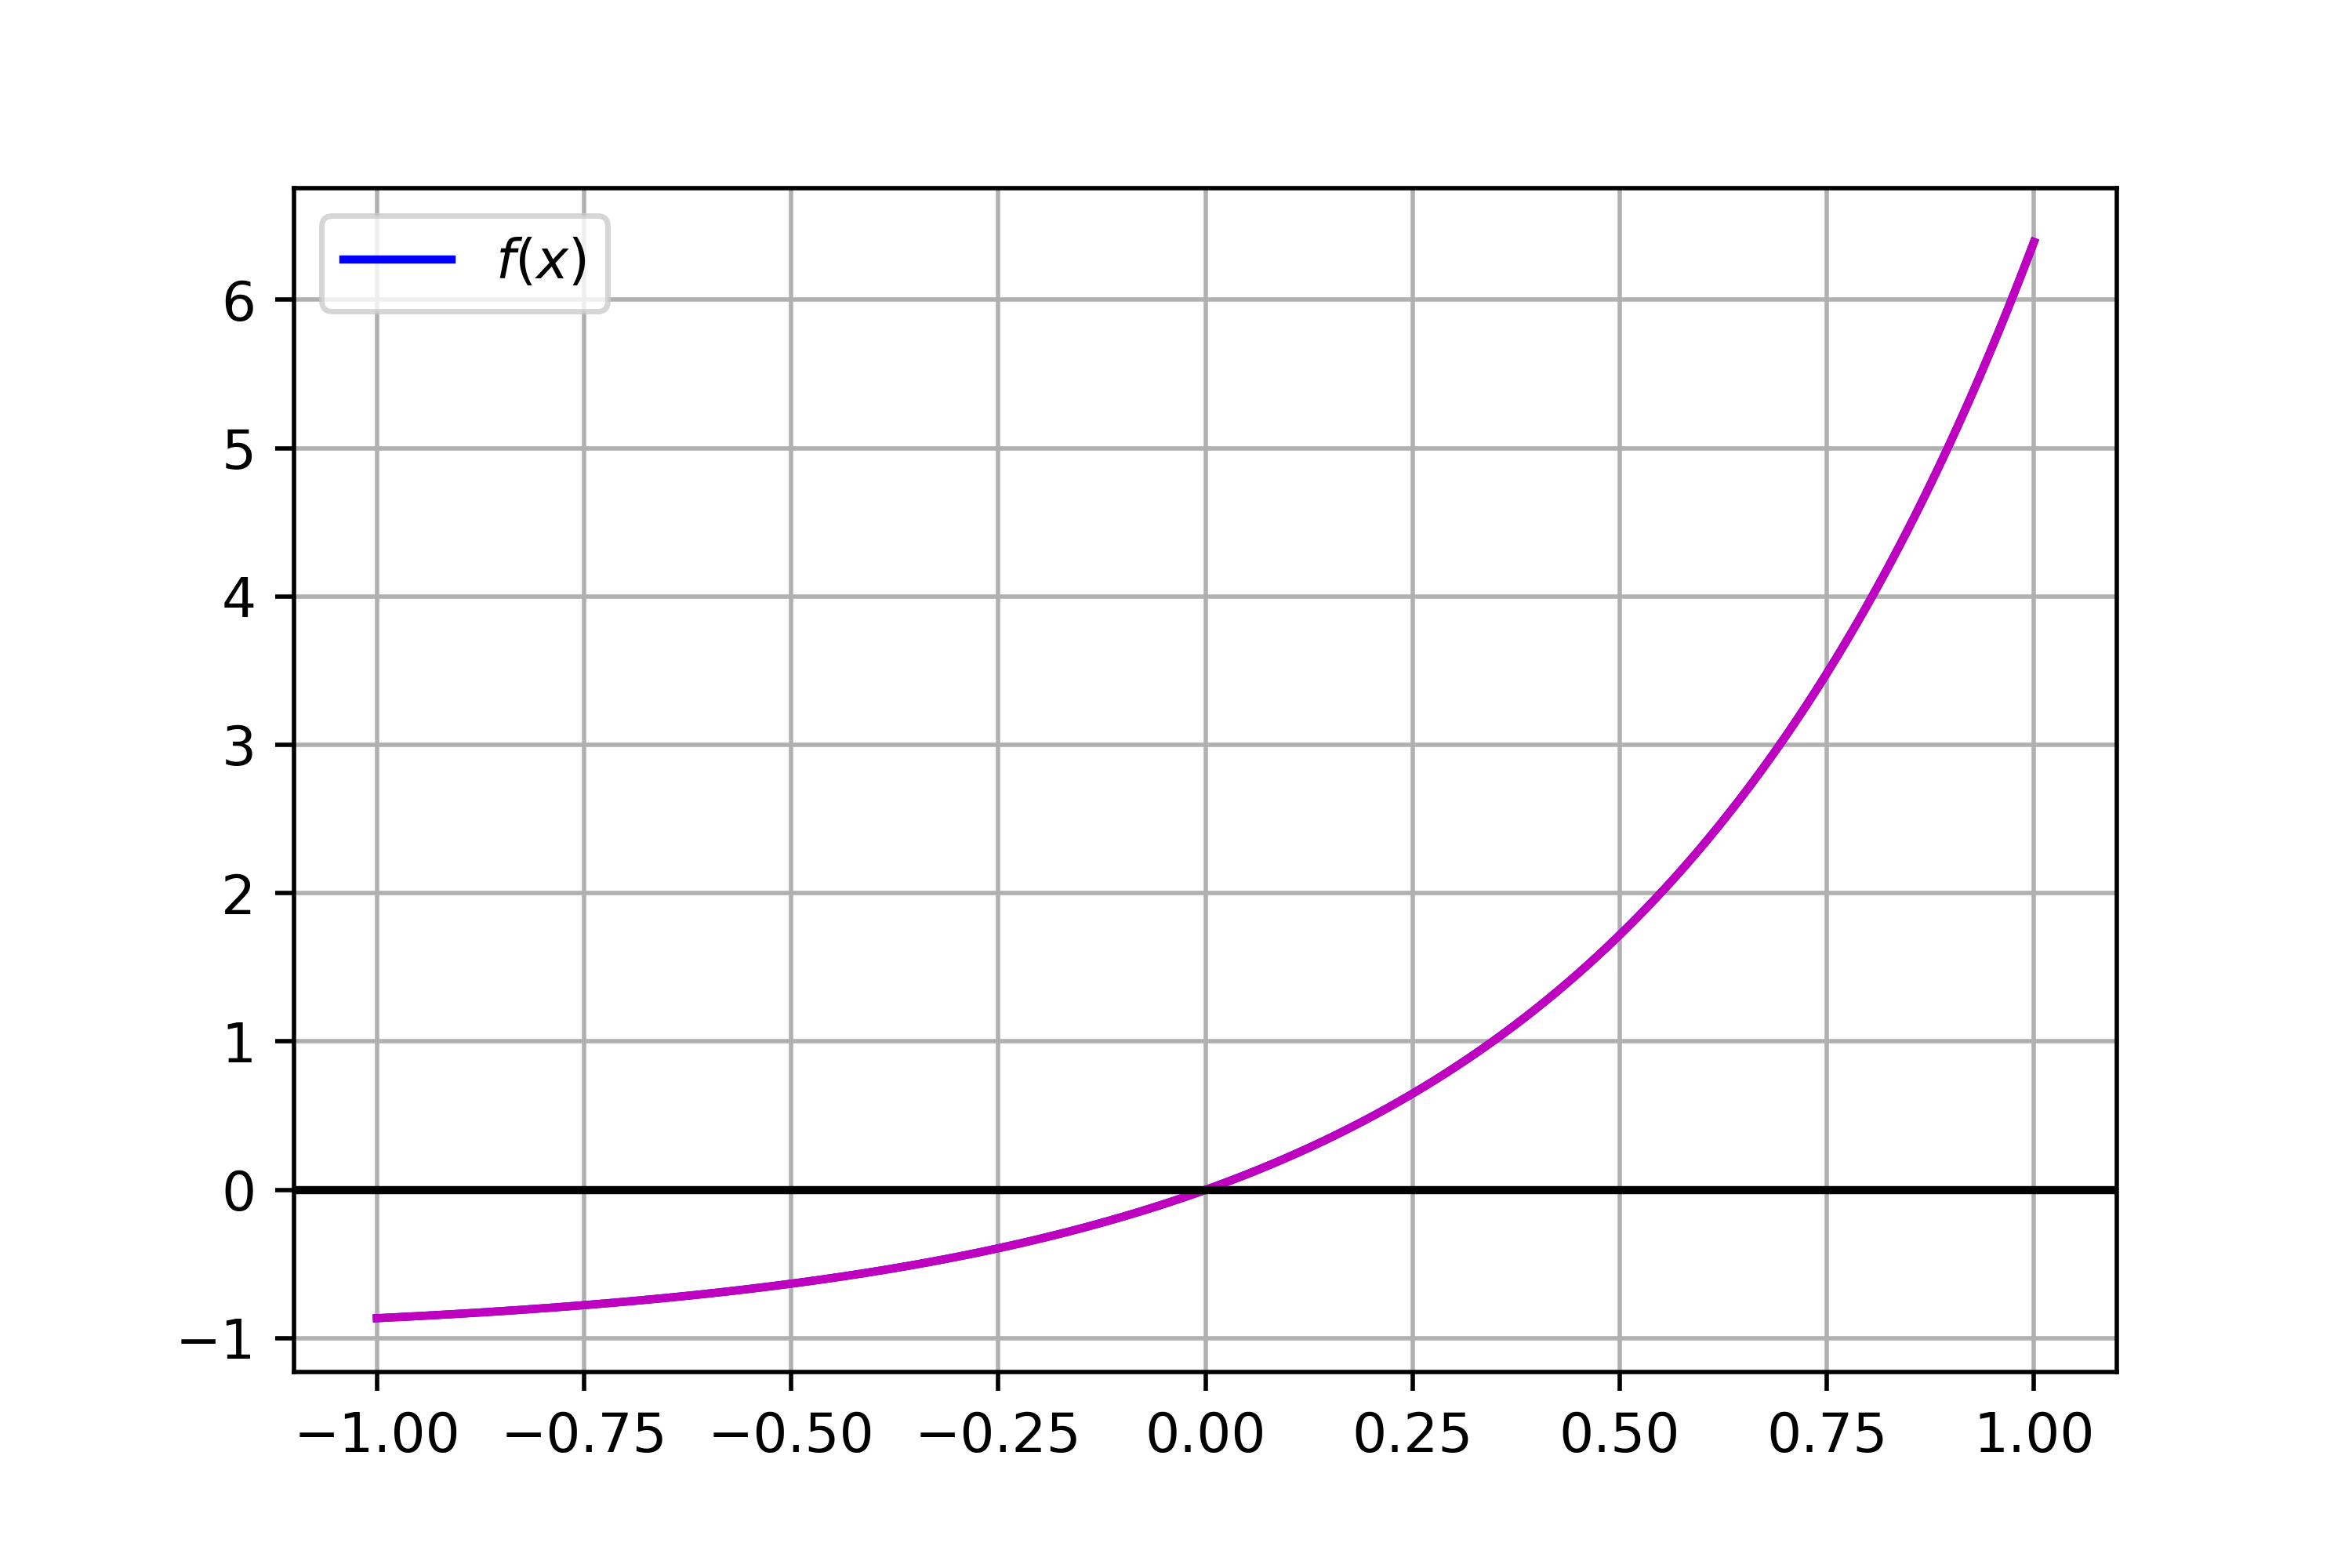
\includegraphics[height=9.5cm]{images/plot_4.3_func.png}

\textbf{Вывод}{
	Увеличение количества членов ряда Тейлора приводит к скачкообразному снижению погрешности и слишком большим степеням многочлена. Как можно видеть, на графике погрешностей до экономизации погрешность избыточно низкая. Экономизация степенного ряда позволяет значительно снизить степень многочлена, сохранив при этом допустимую точность на отрезке.
}
\subsection*{Код программы}
\begin{lstlisting}
import numpy as np
import matplotlib.pyplot as plt
import numpy.polynomial as plnm

f = lambda x: np.exp(2*x) - 1
def Taylor(n):
    power, fact = 1, 1
    while n:
        power, fact = power*2, fact*n
        n -= 1
    return power/fact

def get_n(eps: np.float64) -> int:
    n = 1
    power, fact = 1, 1
    while power/fact >= eps:
        power, fact = power*2, fact*n
        n += 1
    return n-1

def Cheb2Poly(n):
    arr = [0]*n + [1]
    cheb = plnm.chebyshev.Chebyshev(arr)
    poly = plnm.Polynomial(plnm.chebyshev.cheb2poly(cheb.coef))
    return poly

def Economise(P):
    tmpCheb = Cheb2Poly(P.degree())
    PRes = P.cutdeg(P.degree()-1) - P.coef[-1]/(tmpCheb.coef[-1]) * tmpCheb.cutdeg(P.degree()-1)
    return PRes

eps = 1e-8
n = get_n(eps) - 1
a = [Taylor(i) for i in range(1, n+1)]
P0 = plnm.Polynomial([0] + a)
P = [P0]
print(P0.degree(), n)
for i in range(4):
    P.append(Economise(P[-1]))

\end{lstlisting}

\end{document}